%! program = pdflatex

\documentclass[12pt]{article}
\usepackage{geometry} % see geometry.pdf on how to lay out the page. There's lots.
\geometry{a4paper} % or letter or a5paper or ... etc
% \geometry{landscape} % rotated page geometry
\usepackage{epsfig}
\usepackage{amsmath}
\usepackage{natbib}

% See the ``Article customise'' template for come common customisations

\title{Pecube - version 3}
\author{Jean Braun}
\date{\today} % delete this line to display the current date

\renewcommand{\baselinestretch}{1.2}

%%% BEGIN DOCUMENT
\begin{document}

\pagestyle{myheadings}
\markboth{Pecube}{User Guide}

\maketitle
\tableofcontents
\vfill\eject
\begin{abstract}
This is the user guide for version 3 of PECUBE, a finite element code that solves the heat transport equation in three dimensions with the purpose of testing geomorphic and tectonic scenarios against thermochronological data. The code includes the effect of heat conduction and advection (resulting from tectonic transport, such as movement along faults or block uplift/subsidence), heat production by radioactive elements in the crust or resulting from shear heating, the effect of finite amplitude topography. This new version incorporates many changes, including the ability to predict ages below the surface (in a tunnel or in a well), to use surface geometries de- rived from a surface processes model, such as CASCADE, reading an external topography files constructed on an irregular (triangular) discretization, etc. We have also incorporated the Neighbourhood Algorithm of Malcolm Sambridge into PECUBE in its parallelized form to enable the direct in- version of thermochronological data. We have also enriched the library of thermochronological systems that can be predicted, including Richard Ketcham�s fission track algorithm, fission track length distributions for both apatite and zircon, as well as included a simple algorithm to predict age distribution at the surface of the model at any arbitrary time in the past, for direct comparison with detrital age distributions.\end{abstract}

\section{Purpose}

Pecube was initially designed to predict cooling ages for low-temperature chronometers such as apatite fission track or Helium in apatite, mostly in response to land- form evolution. It has been used by a relatively large community who has also contributed to its development through constant requests to see it improved and updated. It has consequently evolved from its original structure to be more user friendly but also more complex in the variety of scenarios that can be tested and thus in its setting up. This new version of the user guide attempts to help the new user to comprehend the code structure and basic functions; it also contains the information that will enable the more confirmed user to use all of its new or �hidden� functions.

When publishing results obtained with PECUBE, please make reference to \citet{Braunsub}.

This new version has benefited from the help of many, including Xavier Robert, Claire Perry, Christoph Glotzbach, Vivi Pedersen and Fr\'ed\'eric Herman, 
\section{Directory structure}

To better organize the use of PECUBE, a directory structure has been adopted that separates the various components into subdirectories: input, output, VTK files, code, data, etc.

The \emph{source} subdirectory contains the Fortran codes of the various subroutines, including those needed by the program \emph{Test} and \emph{Vtk}. These routines should be left unchanged unless you know what you are doing.

The executables are stored in the \emph{bin} subdirectory. To run any of the programs, you must be in the main directory and call the executable by prefixing its name with \emph{bin/}.

The \emph{input} subdirectory contains the two input files described above.

All VTK files are stored in the \emph{VTK} subdirectory.

All output files are stored in the \emph{RUN00} subdirectory (or any other name given in the input file).

All large datasets (topographic and age datasets) are\emph{ }stored in the \emph{data} subdiretory.

This documentation is in the \emph{doc} subdirectory.

\section{Compiling an running PECUBE}

To compile PECUBE , go to the \emph{source} directory: \\
$>$\emph{cd source}\\
and make PECUBE:\\
$>$\emph{make}\\
To compile all other utilities and PECUBE, go to the \emph{source} directory:\\
$>$\emph{cd source}\\
and\\
$>$\emph{make all}.

PECUBE can also be compiled for use on a parallel computer, on which the MPI library has been installed. You will find instructions in the Makefile to do this. Parallelisation will only improve PECUBE runs, not the pre- or post-processors. Note that this option is only meaningful when you run PECUBE in inversion mode. Note also that some compilers will not allow to have an `include' command preceded by a `d' as an indication of a commented line; if this is the case for your compiler, the routine \emph{na.f} will not compile properly. You will need to edit the \emph{na.f} file and remove the `d' in the first column of three lines that start with include 'mpif.h'.

To run Pecube, change the input files in \emph{input/fault\_parameters.txt} and \emph{input/topo\_parameters.txt} to define the setup of your run or experiment, by using your favorite text editor. Beware of not introducing spurious hidden characters by using a fancy word processor such as \emph{WORD} or {Pages}. This would make the input files unreadable by PECUBE. Use a simple text file editor such as \emph{WordPad} or \emph{vi}. Then simply run PECUBE from the main directory, by typing:\\
$>$\emph{bin/Pecube}.\\
Note that this command should not be used if using PECUBE in parallel (NA) mode. In this case, you should refer to your MPI user guide; submitting an MPI process usually looks like:\\
$>$\emph{mpirun -np 8 bin/Pecube}\\
The output is sent to the \emph{RUN00} directory (its exact name can be specified in \emph{input/topo\_parameters.txt}).

Before running PECUBE, you may wish to check that your input files correspond to what you are trying to do (shape of the faults, timing of movement on the faults, surface landform, etc...) To do that, run the Test program from the main directory:\\
$>$\emph{bin/Test}\\
 This will generate VTK files in the \emph{VTK} directory that you can use to check the evolving geometry of the faults and the computed velocity field and the topography.
 
To produce VTK files from the outputs of a simulation, run the \emph{Vtk} program from the main directory:\\
 $>$\emph{bin/Vtk}\\
 This will generate VTK files in the \emph{VTK} directory that you can use to display the temperature field, the ages and the exhumation rate.

You can automate these three actions (Test, Pecube, Vtk) by issuing a single command:\\
$>$\emph{bin/run.sh}\\
Note that this command should not be used when running Pecube in NA mode.

To produce VTK files from the results of an inversion (using NA), run the \emph{ShowNA} program from the main directory:\\
 $>$\emph{bin/ShowNA}\\
 This will generate VTK files in the \emph{VTK} directory that you can use to display the results of the inversion as a set of 3D plot files showing the location of the various runs in paramater space, using as many triplets of axes as required to show all possible combinations. The color of the circles representing the runs is proportional to the misfit value. 

To create a transportable archive of PECUBE, run the \emph{tarngo.sh} shell script from the main directory:\\
 $>$\emph{./tarngo.sh}\\
 This will create a \emph{Pecube.tar.gz} file that contains the content of the source, input and data directories; the other directory are also created in the tar file but they are empty (no solution is stored). This feature is useful if you want to report a bug or a difficulty in running PECUBE. The Pecube.tar.gz file should be relatively small to be sent by email, unless you have very large topographic datasets.
 
\section{Input files}

Two input files are used in this version of PECUBE. They are used by PECUBE to create an input file that has (approximately) the same format as the input file for the first version of PECUBE. This ensures some kind of backward compatibility with the previous versions. The input file for this version (3) is identical to that of version 2, except for a couple of lines added at the end of the \emph{topo\_parameters file.txt} and new options that can be reached by giving negative values to some of the integer parameters. Note that all PECUBE version 2 input files should still work with PECUBE version 3.

Both input files allow the introduction of comment lines (to help describing the input parameters) that start either with a dollar sign or an empty character. These lines are skipped by PECUBE.

\subsection*{Topographic input file}

The first input file is called \emph{topo\_parameters.txt}. It must contain the following lines in the following order:
\begin{itemize}
\item [run] Name of the simulation or name of the directory in which the output of the simulation will be saved; note that the directory must exist prior to the simulation start (type character*5)
\item [topofnme] Name of the input topographic file (DEM) containing a list of $nx$ by $ny$ height values in meters; the DEM starts at the bottom left corner and is given row by row.  If the name of the input file ends with a / character, the topography should be stored in a subdirectory of the \emph{data} directory in the form of a series of file named topo0, topo1 to topo(nstep). This feature is designed to enable the user to use landform geometries obtained from a Landscape Evolution Model (LEM) such as CASCADE. The user must also provide a series of uplift and temp files that contain instantaneous values of the uplift rate and surface temperature computed by the LEM. They should be called uplift0, uplift1 to uplift(nstep) and temp0, temp1 to temp(nstep), respectively. An option also exists to read in irregular topographies (i.e. stored on an irregular, non-rectangular grid). This option is described below. If topofnme is set to Nil the surface topography is assumed to be flat at all times.(type character*(*))
\item [nx0,ny0] dimension of the input DEM;  if nx0 and ny0 are negative, their meaning change: they become the number of nodes and triangles making up the irregular DEM. In that case, the user must also include a file named topofnme.geometry that contains ?nx pairs of coordinates (x and y) in degrees of longitude and latitude, followed by ?ny triplets of node numbers describing the triangular connectivity among the nodes. (type integers)
\item[dlon,dlat] DEM longitude and latitude spacing in degrees (not used when $nx<0$)  (type float )
\item[nskip] skipping factor used to decrease the resolution of the DEM; this parameter is very useful if you wish to test scenarios at low resolution; when constructing the 3D finite element mesh, both nx and ny are divided by nskip (not used when nx < 0) (type integers)
\item [lon0,lat0] longitude and latitude of the bottom left corner of the DEM (type floats)
\item[nstep] the number of times steps in the geomorphic scenario (type integer)
\item[tau] the erosional time scale (the successive topographies given at the various steps are interpolated using an exponential function of time with tau as a decay factor). Most of the time you will wish to turn this off and assume that the change in topography between two time steps is linear; to achieve this use $\tau=0$ (type float)
\item[t,a,o,io] 1 of these per time step+1 (i.e.~you need to include nstep+1 lines like this one), t is the time at which the step starts (in Ma in the past, i.e.~geological time), a is the amplification factor by which the topo read in topofnme will be scaled, o is the offset factor by which it is moved up or down, and io is a flag to determine whether an output (temperature, velocities and detrital ages) is requested at this time (0 for no output, 1 for output) (a and o are not used if $nx<0$)(type 3 floats and 1 integer)
\item[f0,rc,rm,E,n,L,nx,ny] f0 is a flag to allow for flexural isostaty calculations (0 no isostasy, 1 isostasy), rc and rm are the crustal and mantle densities (in kg/m3) respectively, E is young modulus (in Pa), n is Poisson's ratio (dimensionless), L is elastic thickness (in km), and nx and ny the resolutions in both directions of the FFT mesh used to calculate the isostatic flexural response (must be powers of 2)  (type 1 integer, 5 floats, 1 integer)
\item[zl,nz,k,tb,tt,la,pr] zl is the crustal (model) thickness (in km), nz is the resolution in the z-direction, k is the heat diffusivity (in km2/Myr), tb is the temperature at the base of the model (in $^\circ$C), tt is the temperature at the top of the model at mean sea level (in $^\circ$C), la is the lapse rate (in $^\circ$C/km), pr is the heat production (in $^\circ$C/Myr)  (type 1 float, 1 integer, 5 floats)
\item[agefnme] Name of the file containing observed ages (Nil if no data). (type chatacter*(*)). The file should contain the number of observations nobs, then nobs lines containing 
\begin{enumerate}
\item the longitude
\item the latitude
\item the elevation (note that if the age has been obtained from a well, you should input here the depth below the surface as a negative number)
\item apatite He age
\item error in apatite He age
\item apatite FT age
\item error in apatite FT age
\item zircon He age
\item error in zircon He age
\item zircon FT age
\item error in zircon FT age
\item Kspar Ar age
\item error in Kspar Ar age
\item biotite Ar age
\item error in biotite Ar age
\item muscovite Ar age
\item error in muscovite Ar age
\item hornblende Ar age
\item error in hornblende Ar age
\item normalized FT length distribution (apatite) as an array of length 17 (ftld(k) is the proportion of tracks with length between $k-0.5$ and $k+0.5$ microns; the sum of ftld(k) for $k=1,17$ must be equal to 1); if no FT length information use -1 for all 17 values
\end{enumerate}
Negative ages mean no data.
\item[tp,f1,f2,f3,fr] tp is the time of the previous resetting event (for all systems); when a rock does not cross the closure temperature of a given system, its age is set to tp, unless tp is smaller than the time duration of the model run; f1 is a flag that determines which apatite FT routine is used (0 means Peter van der Beek's routine; 1 means Ketcham's routine); f2 is a flag that determines whether to use the differences of the ages (f2=0) or the differences in slopes of the age elevation relationship (f2=1) to construct the misfit function; f3 is a flag that determines whether the faults are advected by one another (f3=1) or not (f3=0); fr is friction coefficient used to multiply an arbitrary stress value of 100 Mpa to compute the heat produced by friction; the heat is calculated as the product of strain rate, stress, and friction coefficient, divided by the specific heat capacity (assumed to be 800 J/C/kg) (type 1 float, 3 integers, 1 float)
\item[f1 to f9] a series of 9 flags to determine which of the ages should be computed; the flags correspond to f1: He in Apatite, f2: He in Zircon, f3: FT in Apatite, f4: FT in Zircon, f5: Ar in Kspar, f6: Ar in Biotite, f7: Ar in Muscovite (White Mica), f8: Ar in Hornblende, f9: Apatite FT length distribution. A value of zero means that the age is not computed (0 will appear in the output file), a value of one means that the age will be computed.
\end{itemize}

\subsection*{Tectonic input file}

The second input file is called \emph{fault\_parameters.txt}. It must contain the following lines in the following order:

\begin{itemize}
\item[nfault] number of faults (this is followed by a series of lines that must be entered for each of the nfault faults) (type integer)
\item[x1,y1,x2,y2] Two lon-lat pairs defining the trace of the fault at the surface. The fault is located to the right of that line (not used if $n<0$, as described below)(type floats)
\item[n] n is the number of points defining the fault; the order in which the points are listed will determine which of the two half spaces defined by the fault moves: it is the one to the right of the fault when going along the fault in the order given in the input file. Note that if n is negative, no fault is assumed and the tectonic velocity field is assumed to be purely vertical and vary as a bi-linear function of space, the value of which is pinned at the four corners of the mesh/DEM (type integer)
\item[r$_i$,s$_i$] n lines containing the r-, s-coordinates of the points defining the fault; if nfault < 0, only one line should be given, containing 4 numbers, i.e.~the value of the velocity field at each of the four corners of the mesh (lower left, lower right, upper left, upper right) (type floats)
\item[nstep] number of time intervals defining the movement on the fault (type integer) 
\item[tstart,tend,velo] nstep lines containing the starting and end times (in geological time; note that if you wish this time interval to start when the previous one finished, input a * (star/times symbol) instead of a time) and a velocity (positive for normal faulting, negative for thrusting) (in case where $n<0$, a positive value means uplift, a negative value means subsidence) (type floats)
\end{itemize}

\section{Faults}

In this section we describe the way faults are defined by a set of linear segments and how the velocity field is determined. This is necessary as there is no uniquely defined solution to this kinematic problem.

\subsection*{Fault geometry}

Let's us first consider the geometry of a single fault as incorporated in PECUBE. It is first defined by a local {\em fault coordinate system} $(r,s)$ that is different from the {\em global three dimensional coordinate system} $(x,y,z)$. As shown in Figure~\ref{fig:coordinatesystem}, this system is fully defined by the position of two points $(x_1,y_1)$ and $(x_2,y_2)$ in the horizontal plane and at the surface $z=z_l$, where $z_l$ is the surface of the model, as defined in PECUBE. The $r$-axis of the fault coordinate system is located to the right of that line (when going along the line from point $1$ to point $2$), the $s$-axis is vertical and the origin is located anywhere along the line at $z=z_l$. To build a fault to the left of a given line, simply invert the order of the two points. That the origin is not strictly defined implies that the fault geometry is two-dimensional and its definition does not depend on its location along the line.

\begin{figure}[htbp]
   \centering
     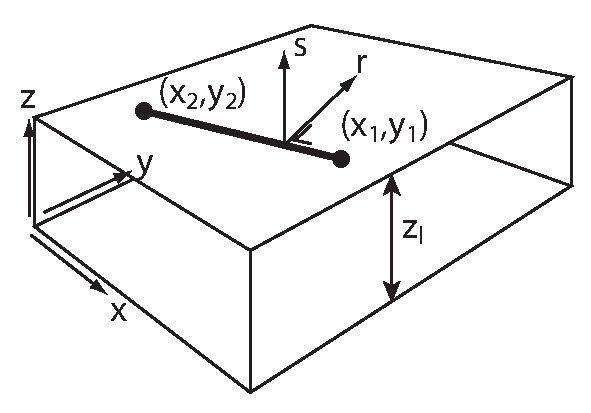
\epsfig{file=coordinatesystem.pdf,width=7cm}
   \caption{The local fault coordinate system and the global PECUBE system.}
   \label{fig:coordinatesystem}
\end{figure}

In the $(r,s)$ plane, the fault is defined through a series of n connected points $(r_i,s_i)$. The segments connecting the points define the fault trace in the $(r,s)$ plane. The end segments are assumed to continue indefinitely.

The order in which the nodes are given is important: it determines which half-space (there is one on either side of the fault) moves with respect to the fault. When moving along the fault in the order in which the nodes are given, the half space that moves with respect to the fault is the one to the right of the fault. The other half-space is fixed. If one wishes to make it move too, one needs to define a second fault of the same geometry but with the nodes given in the reverse order. 

The velocity of the half space along the fault $v_0$ is imposed along the fault surface and its sense is given by the sign of $v_0$: normal faults have a positive velocity, thrust fault a negative velocity.

Finally the fault is not defined (the velocity is nil) for regions outside of the infinite strip perpendicular to the two points $(x_1,y_1)$ and $(x_2,y_2)$.

\subsection*{Velocity field}

The velocity field is calculated from the geometry of the various faults and their respective velocities. The algorithm is rather simple and easy to implement.

A two-dimensional velocity field is first calculated in the $(r,s$)-plane and later rotated and translated in the proper location in the $(x,y,z)$-space.

First, one considers each segment individually. In the region defined by the fault segment and its normals at each end of the fault segment, the velocity is set parallel to the fault with amplitude $v_0$. Two situations have to be considered next, when considering successive fault segments: they either form an acute (closed) or obtuse (open) angle (see Figure~\ref{fig:segments}).

\begin{figure}[htbp]
   \centering
     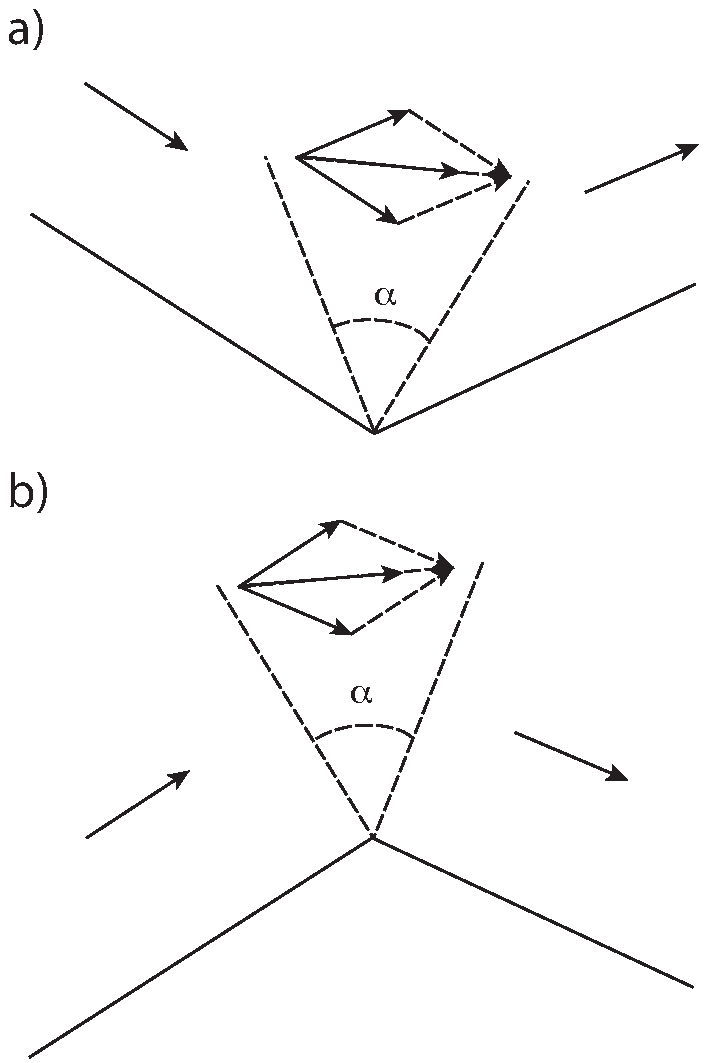
\epsfig{file=segments.pdf,width=7cm}
   \caption{Imposed velocity field in the vicinity of a kink in the fault.}
   \label{fig:segments}
\end{figure}

In the first case (acute angle), the direction of the velocity vector in the `overlapping' region is set to the mean of the directions of the two segments (using the definition of the sum of two vectors to calculate the mean); its amplitude is:
\begin{equation}
v'_0=v_0\frac{\cos\alpha}{\cos\frac{\alpha}{2}}
\end{equation}
where $\alpha$ is the angle made by the the two normals to the segments. In the second case, the direction is also the mean of the directions of the segments, but the amplitude is given by:
\begin{equation}
v'_0=v_0\frac{1}{\cos\frac{\alpha}{2}}
\end{equation}
The amplitudes are obtained by imposing continuity of the normal component of the velocity across the boundaries defining the various regions, to ensure mass conservation.

\subsection*{More than one fault}

When considering the compounded movement of several faults, one must take into account the advection of the position (and potentially the geometry) of one fault with respect to the other. In this new version of PECUBE, the faults are advected by considering which fault is on the `moving side' of all the others and applying the corresponding displacement (product of the velocity by the time step) to each of the points defining the fault. Note that this works well when the fault being displaced lies within a uniform velocity field and straight segments remain straight; but it breaks down when the fault is displaced by a non uniform velocity field (such as in the vicinity of a kink). This is thus not recommended or it is requested that to maintain some kind of accuracy, the fault being displaced ought to be discretized by a large number of segments.

\section{Detrital ages}

PECUBE's main purpose is to compute synthetic thermochronological ages from given/imposed tectonic and geomorphic scenarios. To compute ages, one needs to estimate the temperature history of points that end up at the surface of the model at the end of a simulation. This requires a two-pass algorithm. Firstly, one places points at the surface at $t=$now and, using the set tectonic velocities (and the component from the isostatic rebound if necessary), one works out the original position of those points by playing the tectonic scenario backwards. Secondly, during the temperature (forward) calculations, the points are gradually advected towards their final position recording their temperature on the way. At the end of the simulation the ages are calculated from the $T-t$-paths.

To predict detrital ages, one must perform this calculation for points that end up at the surface of the model at set times in the past. In this new version of PECUBE, the number of particles/points being tracked is equal to the number of points defining the surface ($nsurf$) times the number of time steps ($nstep$). During the first pass of the calculations, these points are located at the surface at the set times (when one needs a detrital age distribution) and advected backwards. During the forward model calculations, the points are advected towards the surface; at the set times, they are `frozen' in their final position and their computed $T-t$-paths are used to calculate the detrital ages.

Note that the predicted detrital ages must be weighted by the predicted/imposed exhumation rate at the time, before they can be compared to observed detrital distributions.

\section{Chronometers}

In this new version of PECUBE, eight thermochronometers are simulated: U-Th/He in apatite and zircon, Fission Track in apatite and zircon and K-Ar in Kspar, biotite, white mica (muscovite) and hornblende. The diffusion parameters used are those given in \citet{BraunBook}; a choice of annealing parameters are available for the fission track simulations (see the corresponding routines \emph{Mad\_Trax.f} and \emph{Mad\_Trax\_Zircon.f}). In this version we are providing the choice of two routines for FT ages in apatites based on \citet{vanderbeekthesis} or \citet{Ketcham2000}. We have also included the possibility of predicting FT length distributions for both apatite and zircon and comparing them to observed distributions, that must be included in the observation file.

\section{Output}

The ages are given as Text files (\emph{Ages001.txt}, \emph{Ages002.txt}, $\cdots$, \emph{Agesnnn.txt}) corresponding to each time steps requested. The ages, the geometry of the surface and the exhumation rate are also stored in a binary file (\emph{Ages.out}) that can be used to produce VTK files (\emph{Ages001.vtk}, \emph{Ages002.vtk}, $\cdots$, \emph{Agesnnn.vtk}) by using the \emph{Vtk} program.\emph{Vtk} also produces VTK files (\emph{Pecube001.vtk}, \emph{Pecube002.vtk}, $\cdots$, \emph{Pecubennn.vtk}) of the temperature field and the velocities from another binary output file called \emph{Pecube.out}.

\section{Inversion or NA mode}

In this new version of PECUBE, we have included the basic set of NA (Neighbourhood Algorithm of \citet{Sambridge1999a}. This algorithm will try to find the optimum values of given parameters of the model that will minimize a misfit function defined by the difference between observed ages and predictions. Note that data (ages) is necessary for this option to work. Two misfit functions can be used (see above).

To enable this feature, you simply need to replace the value of the parameter you wish to invert for (in the \emph{fault\_parameters.txt} or \emph{topo\_parameters.txt} files) by a range of values separated by a colon (:). NA will search within that range.

You also need to create or modify the file called \emph{na.in} in the \emph{NA} subdirectory to include:
\begin{itemize}
\item[i1]          : Algorithm type (NA or Uniform MC: 1=MC,0=NA)
\item[i2]        : Maximum number of iterations
\item[i3]         : Sample size for first iteration
\item[i4]         : Sample size for all other iterations
\item[i5]         : Number of cells to re-sample 
\item[i6,i7]  : Use Quasi random number generator ? (y/n);random seed 
\item[i8]         : Type of initial sample (0=random;1=read in a NAD file)
\item[i9]         : Output information level (0=silent,1=summary info,2=1+models)
\item[c1]         : Turn timing mode on ? (y/n)
\item[c2]         : Turn debug mode on ? (y/n)
\end{itemize}

\section{Examples}

\subsection*{Example 1: King Canyon}

In this example we will use the DEM around Kings Canyon, California, as well as the He in apatite dataset published in \citet{Houseetal1998}. We will run two distinct scenarios, one in which the present-day topography is assumed to be old (i.e.~it formed by linear decay of a larger amplitude topograpyh that was created 90 Myr ago) and one in which it is assumed to be young (created in the last 5 Myr). In both scenarios, we will rapidly exhume rocks (at 1 km/Myr) during an orogenic event that spans the 110 to 90 Ma time span, and then very slowly (at 0.03 km/Myr) during the remaining 90 Myr. Note the use of the `*' symbol to specify the start of the second exhumation period as equal to the end of the previous period (90 Myr).

First go in the input directory and copy the \emph{topo\_parameters.txt.KingCanyon} file to \emph{topo\_parameters.txt}:\\
$>$\emph{cp topo\_parameters.txt.KingCanyon topo\_parameters.txt}\\
as well as the fault\_parameters.txt.KingCanyon to fault\_parameters.txt:\\
$>$\emph{cp fault\_parameters.txt.KingCanyon fault\_parameters.txt}

Go back to the main \emph{Pecube} directory and run PECUBE:\\
$>$\emph{bin/run.sh}\\

This should take a few minutes on a reasonably new computer. Once the run is finished, you can use a VTK viewer (PARAVIEW, for example) to display and inspect the various VTK files created by PECUBE.

In Figures \ref{fig:KingsCanyon1} and \ref{fig:KingsCanyon2}, we show the results of the first and second model runs, respectively, in terms of the He in apatite ages contoured on the topography.

\begin{figure}[htbp]
   \centering
     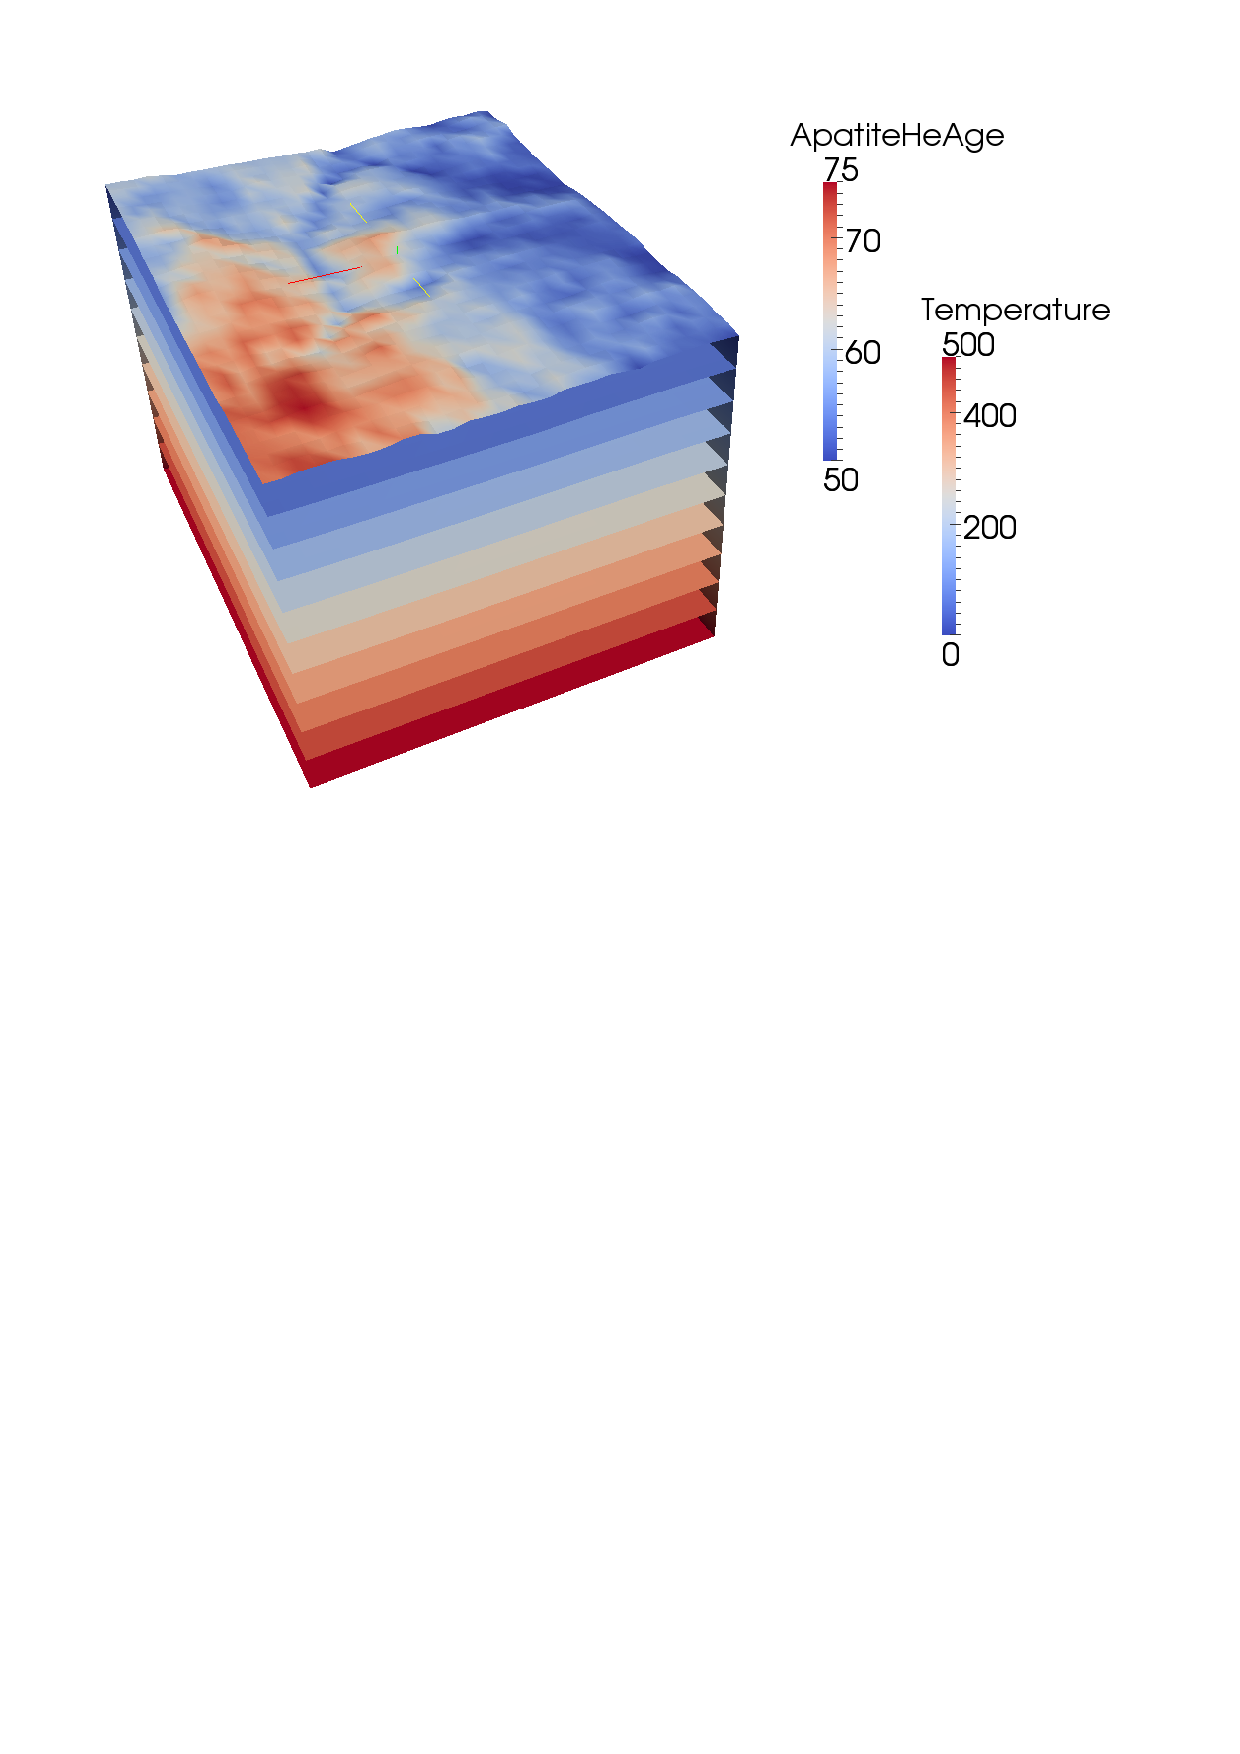
\epsfig{file=PecubeKingsCanyon1,width=15cm}\\
   \caption{Results of a PECUBE experiment in which the relief of Kings Canyon is assumed to be old.}
   \label{fig:KingsCanyon1}
\end{figure}
\begin{figure}[htbp]
   \centering
     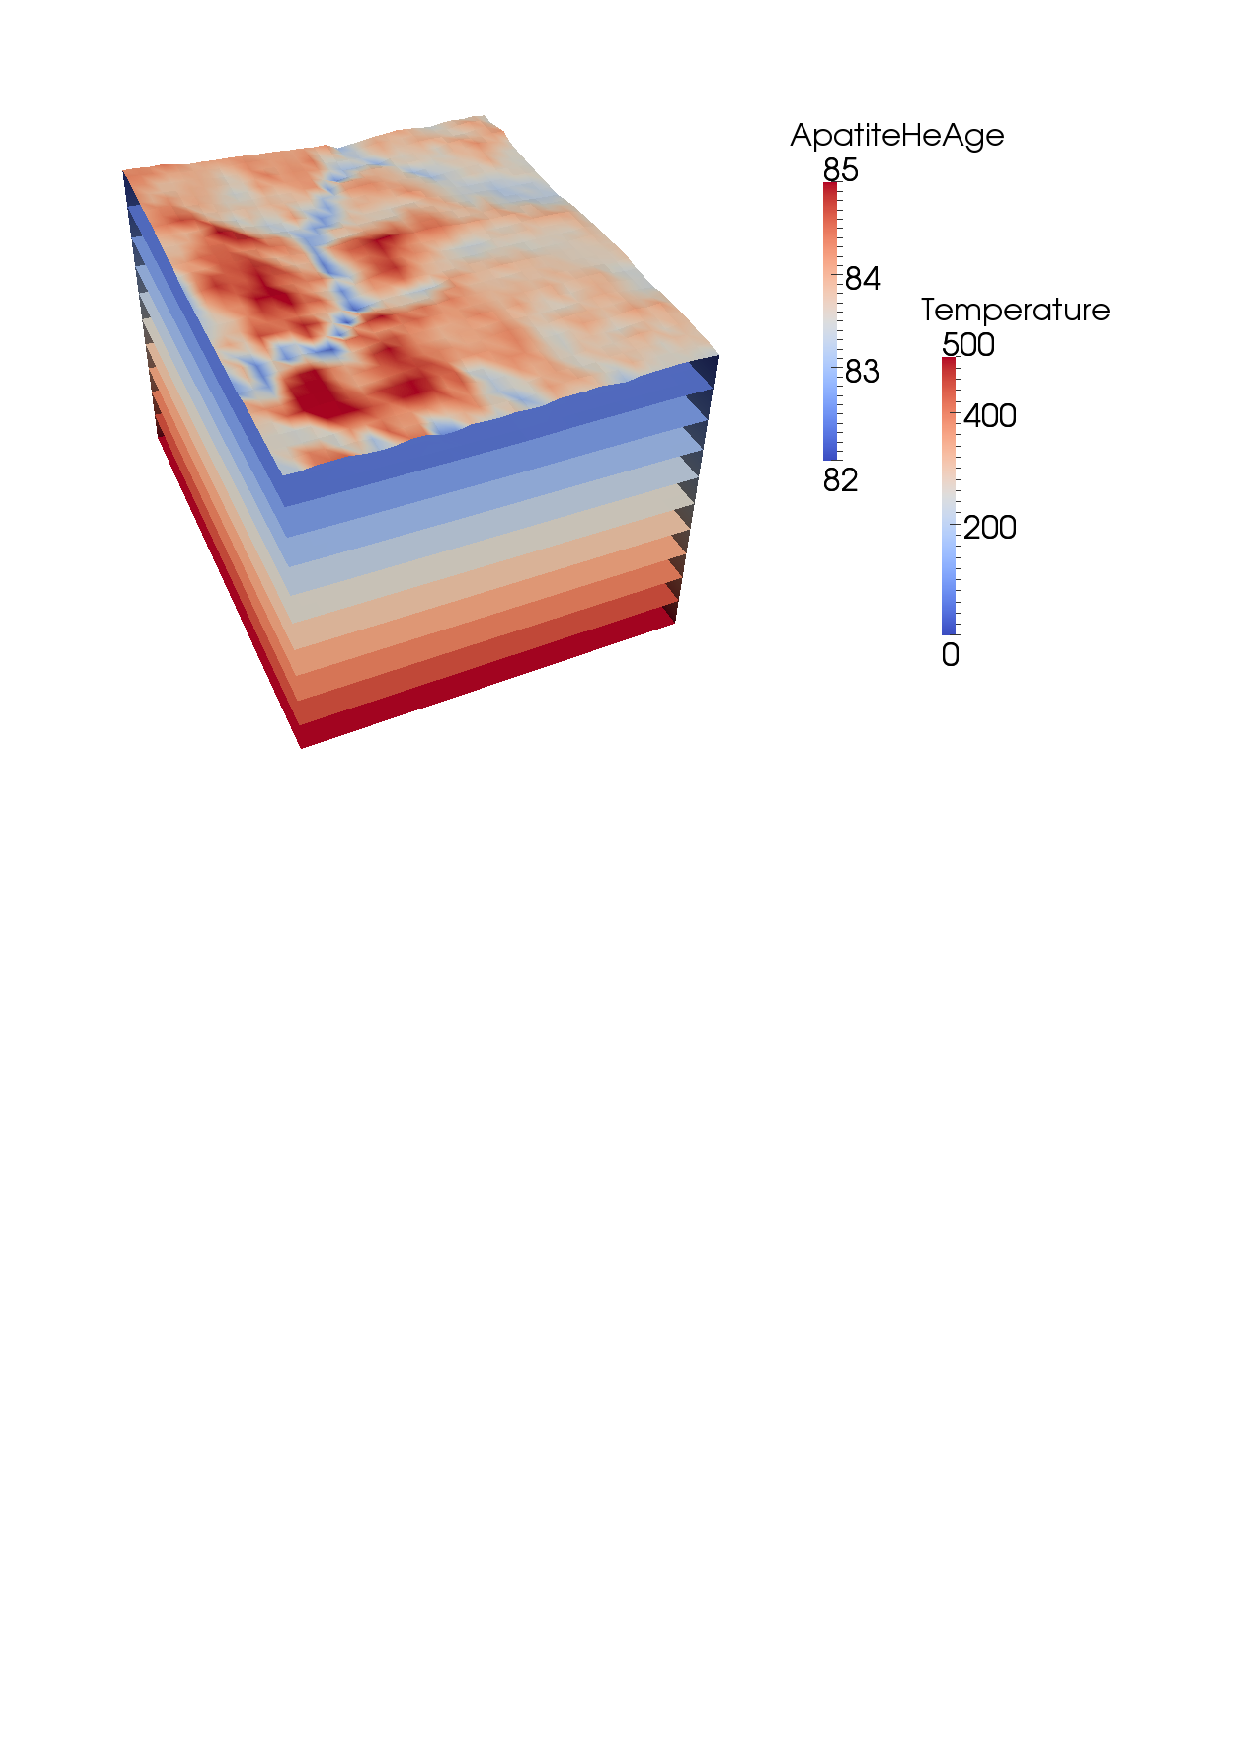
\epsfig{file=PecubeKingsCanyon2,width=15cm}
   \caption{Results of two separate PECUBE experiments in which the relief of Kings Canyon is assumed to be young.}
   \label{fig:KingsCanyon2}
\end{figure}

Now you should change the \emph{topo\_parameters.txt} file and replace the value of the basal temperature by a range of values (400:600, for example) and the \emph{fault\_parameters.txt} file to change the timing of the end of the tectonic episode from 100:70 and the exhumation velocity in the slow exhuming episode from 0.02:0.04. Alternatively you can copy the \emph{fault\_parameters.txt.Inversion} to \emph{fault\_parameters.txt} and the \emph{topo\_parameters.txt.Inversion} to \emph{topo\_parameters.txt}.

We advise you to compile PECUBE using MPI-enabled compilers and run this example by using the following command

$>$\emph{mpirun -np 8 bin/Pecube}

replace 8 by the sample size per iteration defined in \emph{na.in} to optimize the run.

\begin{figure}[htbp]
   \centering
     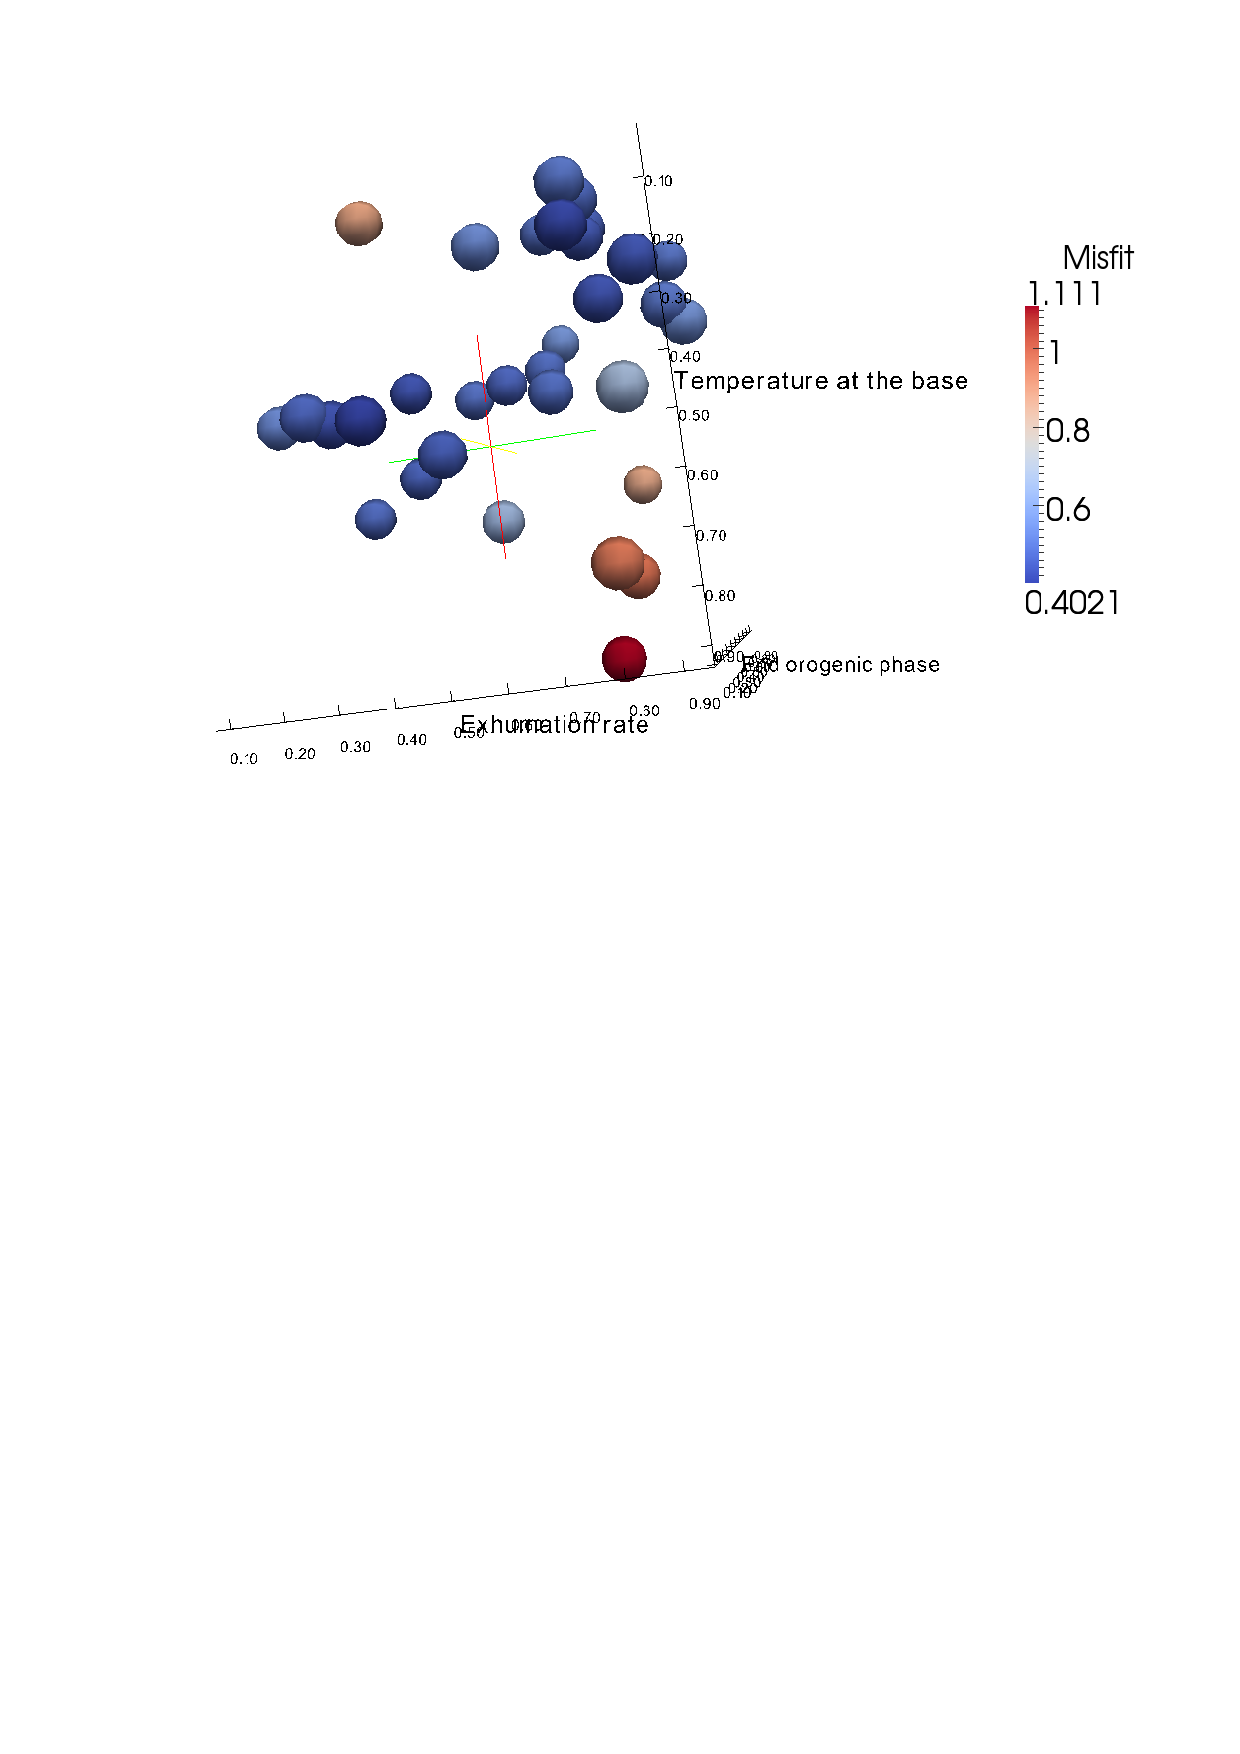
\epsfig{file=PecubeKingsCanyonNA,width=15cm}\\
   \caption{Results of an inversion run using the KingsCanyon dataset to compute the misfit.}
   \label{fig:KingsCanyonNA}
\end{figure}

\subsection*{Example 2: Whataroa Valley}

The second example illustrates the use of a fault to define the tectonic velocity field. The two input files are \emph{topo\_parameters.txt.Whataroa} and \emph{fault\_parameters.txt.Whataroa}. They use a topographic dataset from around the Whataroa Valley in the central section of the South Island, New Zealand, where the rapid relative motion between the Pacific and Australian plates is accommodated by the Alpine Fault.

Note how the fault surface trace is defined by pairs of two pairs of longitude-latitude coordinates corresponding to the extremities of the line defining the width of the fault segment. Note that the order in which these points are given defines where the fault dips (always to the right of the line), which means that, in this case, the southwestern corner is given first. The fault geometry is then defined by a series of distance-depth pairs in a direction perpendicular to the fault trace. Note first that the depth are given as negative numbers, and second, that the order in which the points defining the fault segments are given determines which of the two blocks (the footwall or the hanging wall) moves. By convention, it is the block to the right of the fault (when moving along the fault in the order given in the input file) that moves. In this case we want the hanging wall to move; consequently, we give the points from the deepest to the shallowest. Here we define the fault as made of two segments defined by three distance-depth points: a first horizontal segment at a depth of 25 km and a second segment dipping at approximately 60$^\circ$ to the east.

The velocity on the fault is finally given as a negative number to indicate that it is a thrust fault. The velocity field corresponding to this geometry is computed internally by PECUBE as explained above. It consists of three regions: to the right (east), along the flat/horizontal segment of the fault, the velocity is horizontal, to the left (west), above the dipping segment of the fault, the velocity is parallel to the fault, i.e.~dipping at 60$^\circ$, and in an intermediate triangular region, the velocity is the mean of the velocities in the other two regions. This velocity field is shown in Figure~\ref{fig:NZFault} along a plane perpendicular to the fault.

\begin{figure}[htbp]
   \centering
     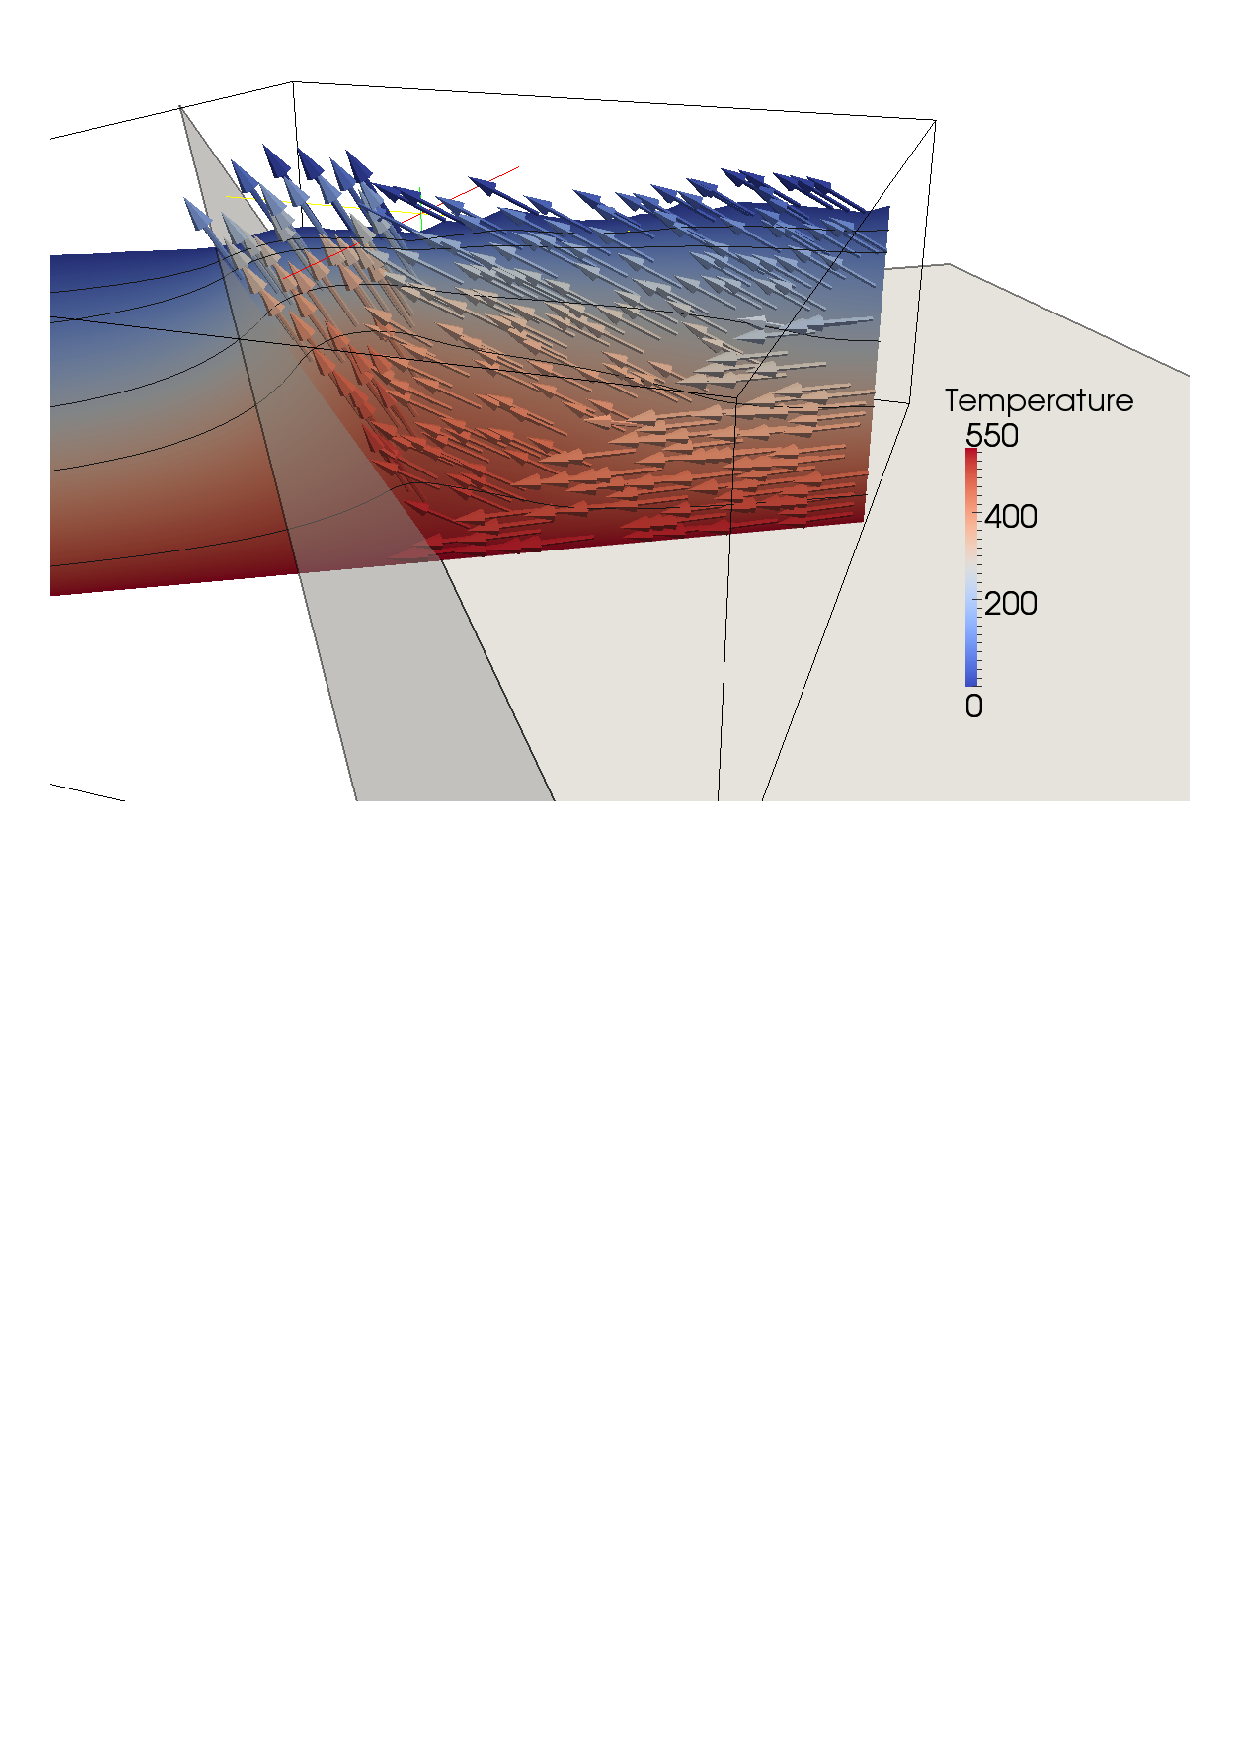
\epsfig{file=PecubeWhataroa4,width=15cm}\\
   \caption{Geometry of the fault used in the second example and corresponding velocity field displayed along a plane perpendicular to the fault trace.}
   \label{fig:NZFault}
\end{figure}

We imposed that the present day convergence started about 6 Ma and that the topography started growing at about the same time to reach its present-day value at about 4 Ma. Note, however, that, in the current version of PECUBE, no strike-slip motion can be imposed on faults. This is because the strike-slip component of deformation does not influence much the distribution of cooling ages along a linear structure.

Finally, it is worth noting that we imposed a timing of 100 Ma for the previous tectonic event. We have also limited the number of age/systems being computed to fission track in apatite only (see the flags at the bottom of the input \emph{topo\_parameters.txt} file).

Results of the computations are shown in Figure~\ref{fig:NZResults}.  Note how the isotherms are compressed towards the surface in the vicinity of the fault (on the upthrow side) as a result of heat advection by the imposed velocity field (shown in Figure~\ref{fig:NZFault}). Consequently the FT ages are very young near the fault (i.e.~close to 0 Ma, as observed by \citet{Tippett1993}) and along most of the western side of the orogen. Along the eastern flank, ages get older and reach pre-Alpine values of approximately 100 Ma, as imposed in the input file.

\begin{figure}[htbp]
   \centering
     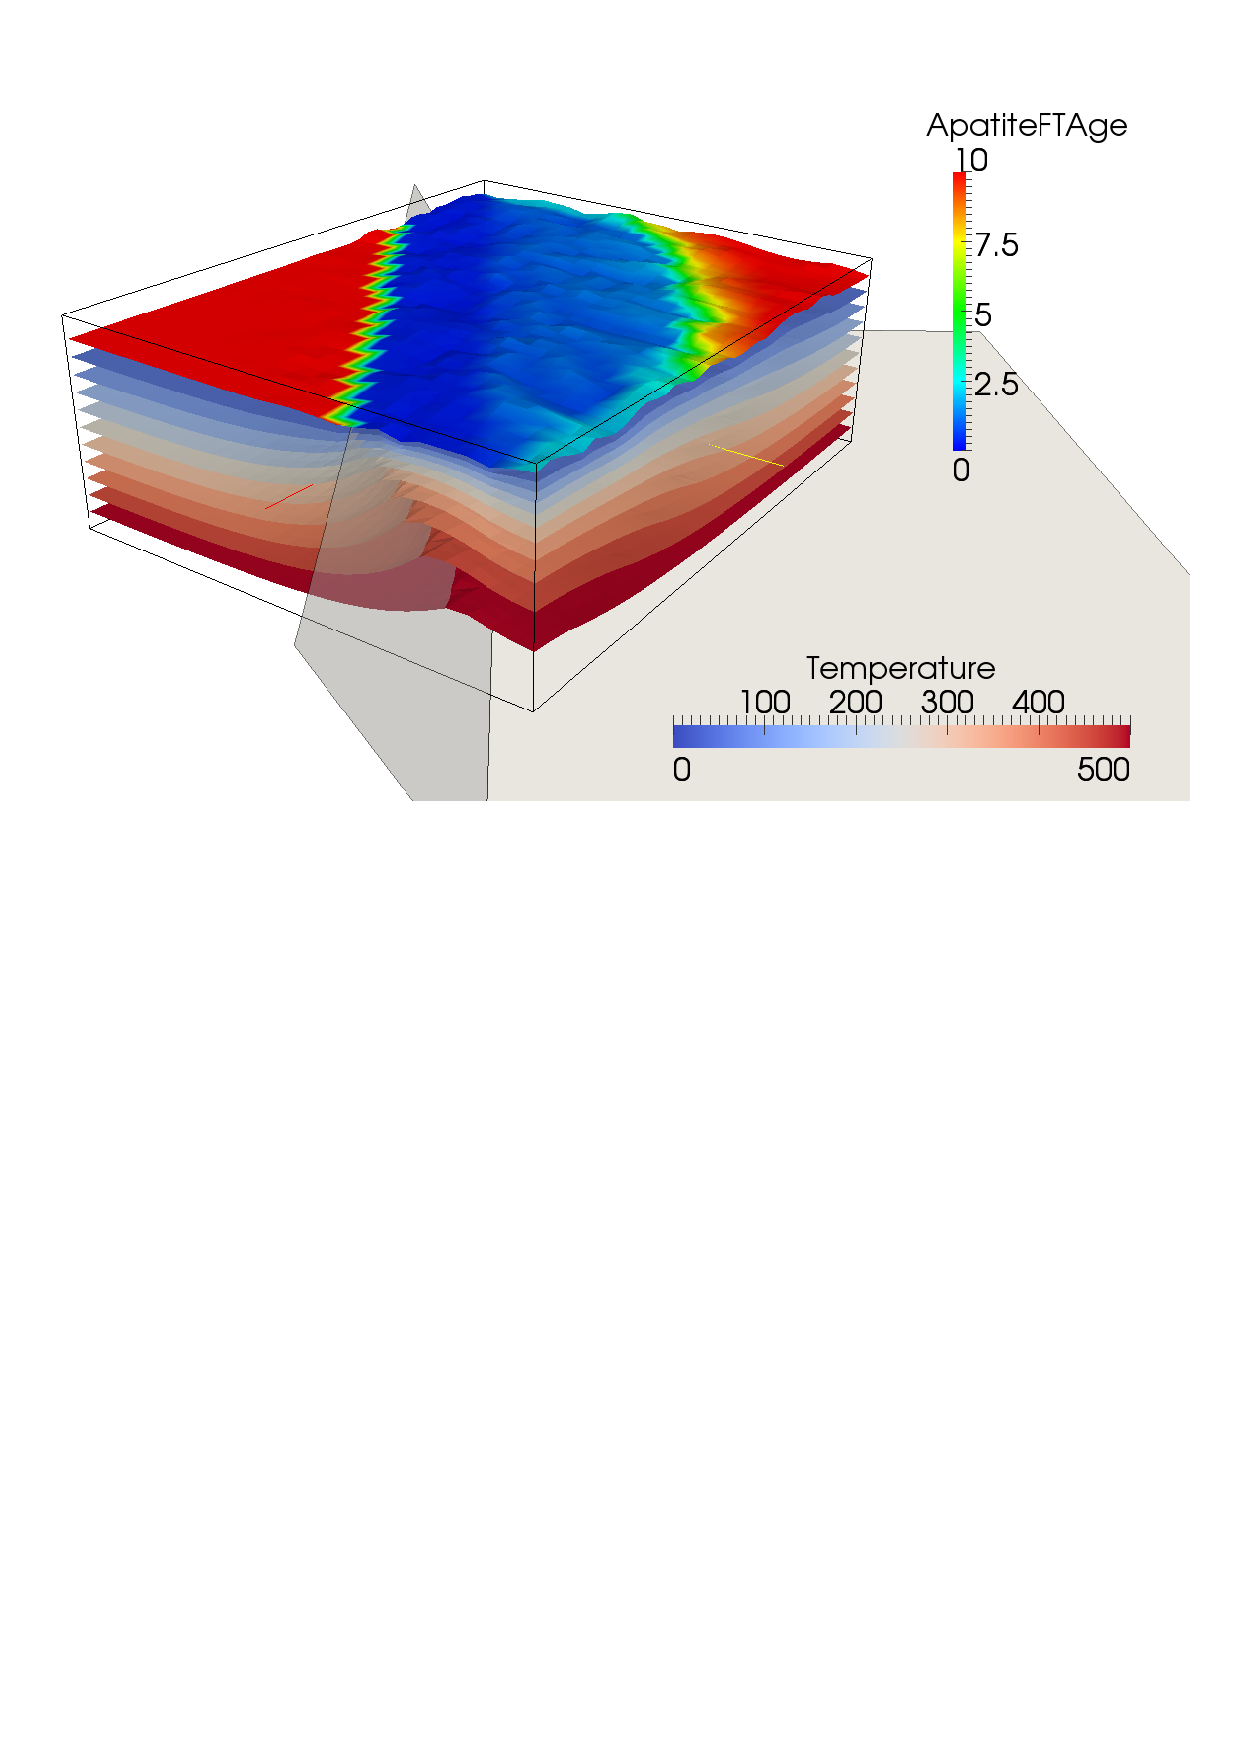
\epsfig{file=PecubeWhataroa1,width=15cm}\\
   \caption{Computed Apatite fission track ages, temperature field and imposed fault geometry.}
   \label{fig:NZResults}
\end{figure}

We suggest to the user to modify the input file to include frictional heating along the fault by setting the coefficient of friction at 0.1, for example, to represent a relatively weak fault. The new solution is shown in Figure~\ref{fig:NZFriction}. The heat produced by friction along the fault causes a further upwarping of the isotherms on either sides of the fault.

\begin{figure}[htbp]
   \centering
     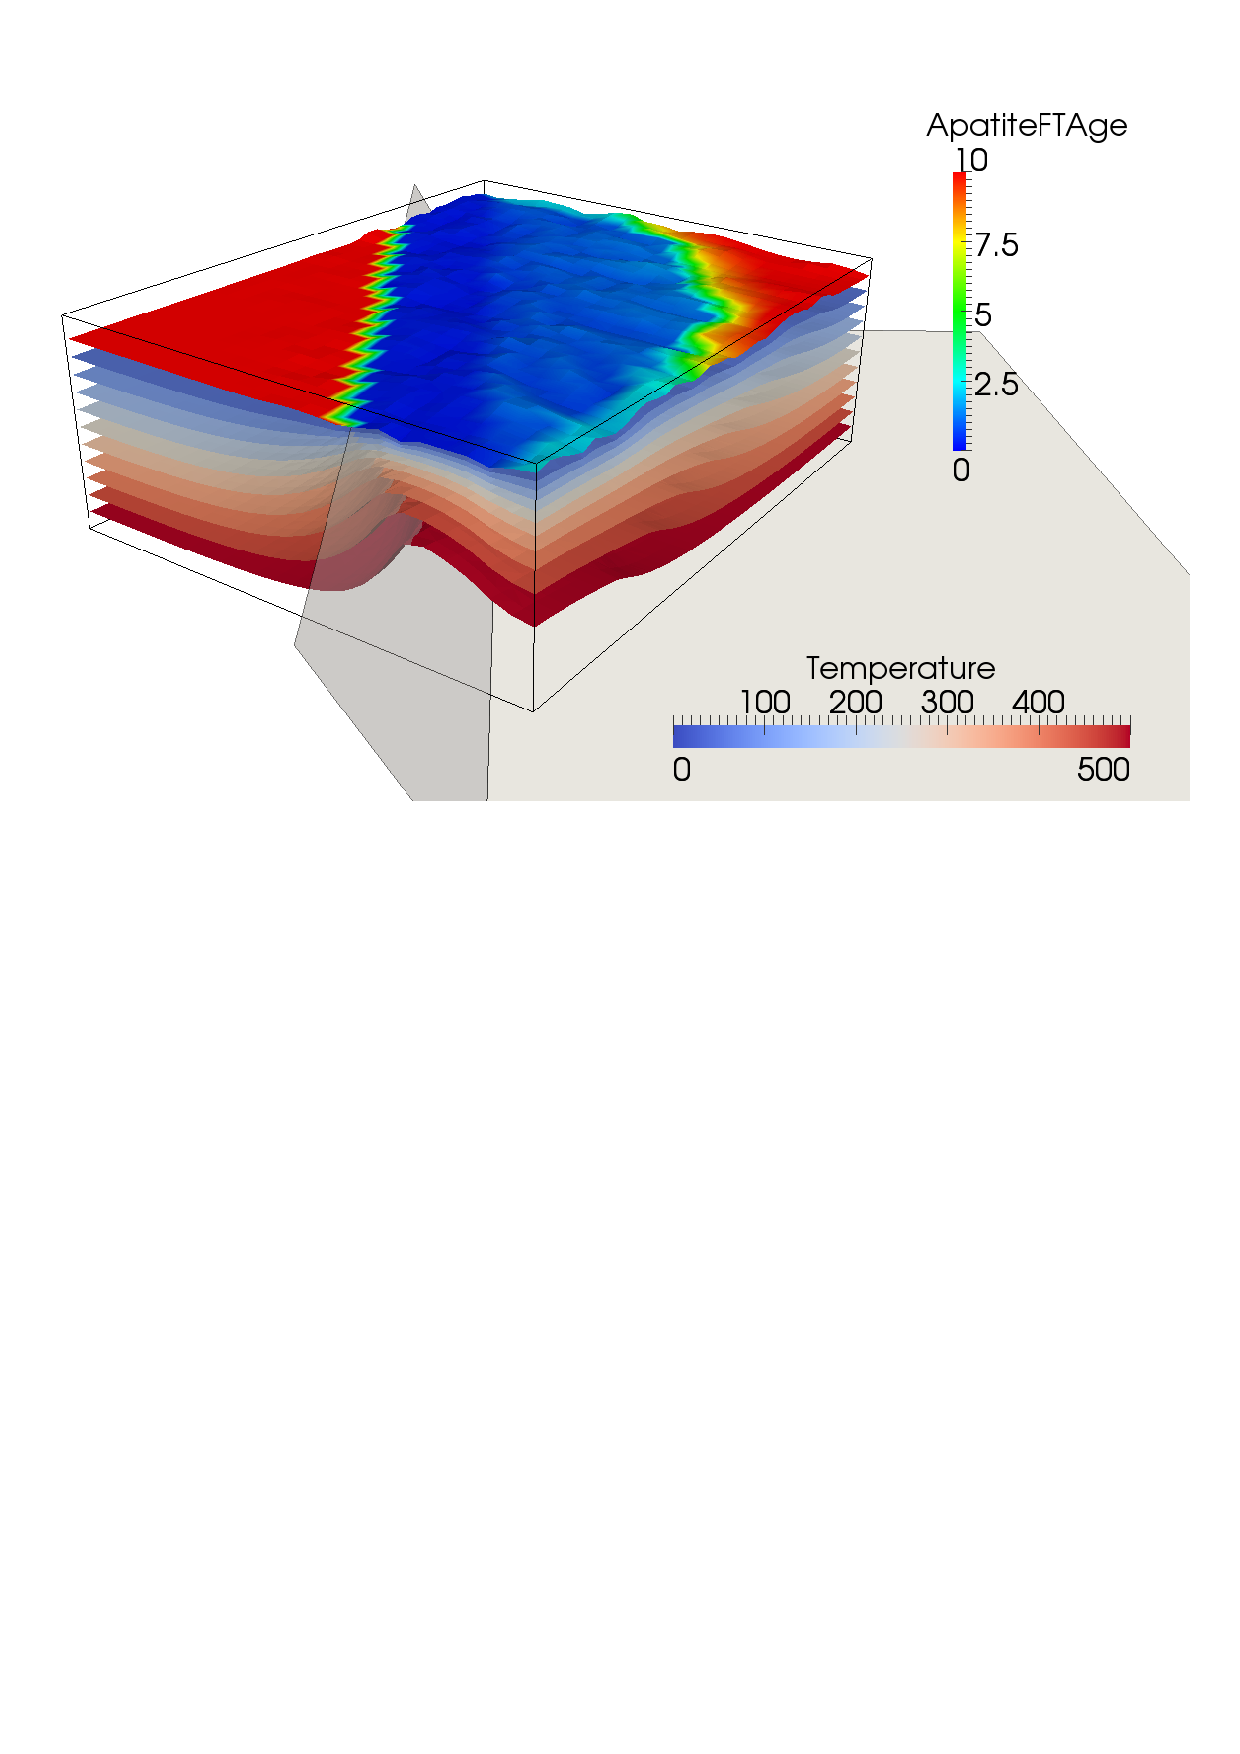
\epsfig{file=PecubeWhataroa5,width=15cm}\\
   \caption{Computed Apatite fission track ages, temperature field and imposed fault geometry. Same as Figure~\ref{fig:NZResults} but including frictional heat.}
   \label{fig:NZFriction}
\end{figure}

\subsection*{Example 3: Synthetic landscapes}

In this third example, we use synthetic landscapes produced by the CASCADE software as input topographic files for PECUBE. This requires a series of topographic, uplift and surface temperature files generated from the output of a CASCADE run. To create these files, we have written a simple FORTRAN code named \emph{cascade2Pecube.f90} that can be found in the source subdirectory. If using another surface processes model (SPM) to produce the synthetic landscapes, the user will need to modify this Fortran code to accept the output created by the other SPM.

Output files (connectivity, geometry, uplift rate, topography) from a cascade run need to be stored in the \emph{cascade\_output} subdirectory before running \emph{bin/cascade2Pecube} from the main Pecube directory. You will be prompted for a directory file name that will need to create in the data directory before running cascade2Pecube. This will create as many topo, temp and uplift files as there are time steps in the CASCADE output files. You will then need to modify the \emph{topo\_parameters.txt} file to indicate the number of time steps and their associated times. Parameters such as the skip factor or the spacing in degrees will not be used. Set the bottom left corner of the mesh to longitude-latitude (0,0). Use the \emph{topo\_parameters.txt.Cascade} as a template.

The \emph{fault\_parameters.txt} files should not be used to define an additional uplift/velocity field. Make sure that the number of faults is set to zero, right at the top of the file.

We will use this example to compute histograms of age distribution at the various intermediate time steps 0, 1, 2, 3, 4 and 5 Ma (corresponding to \emph{Ages010.txt}, \emph{Ages008.txt}, \emph{Ages006.txt}, \emph{Ages004.txt}, \emph{Ages002.txt} and \emph{Ages000.txt}, respectively) for the He in apatite thermochronometer. These are shown in Figure~\ref{fig:Detrital}. They show a relatively constant lag time \citep{Bernet2004} for the past 3-4 Myr.

\begin{figure}[htbp]
   \centering
     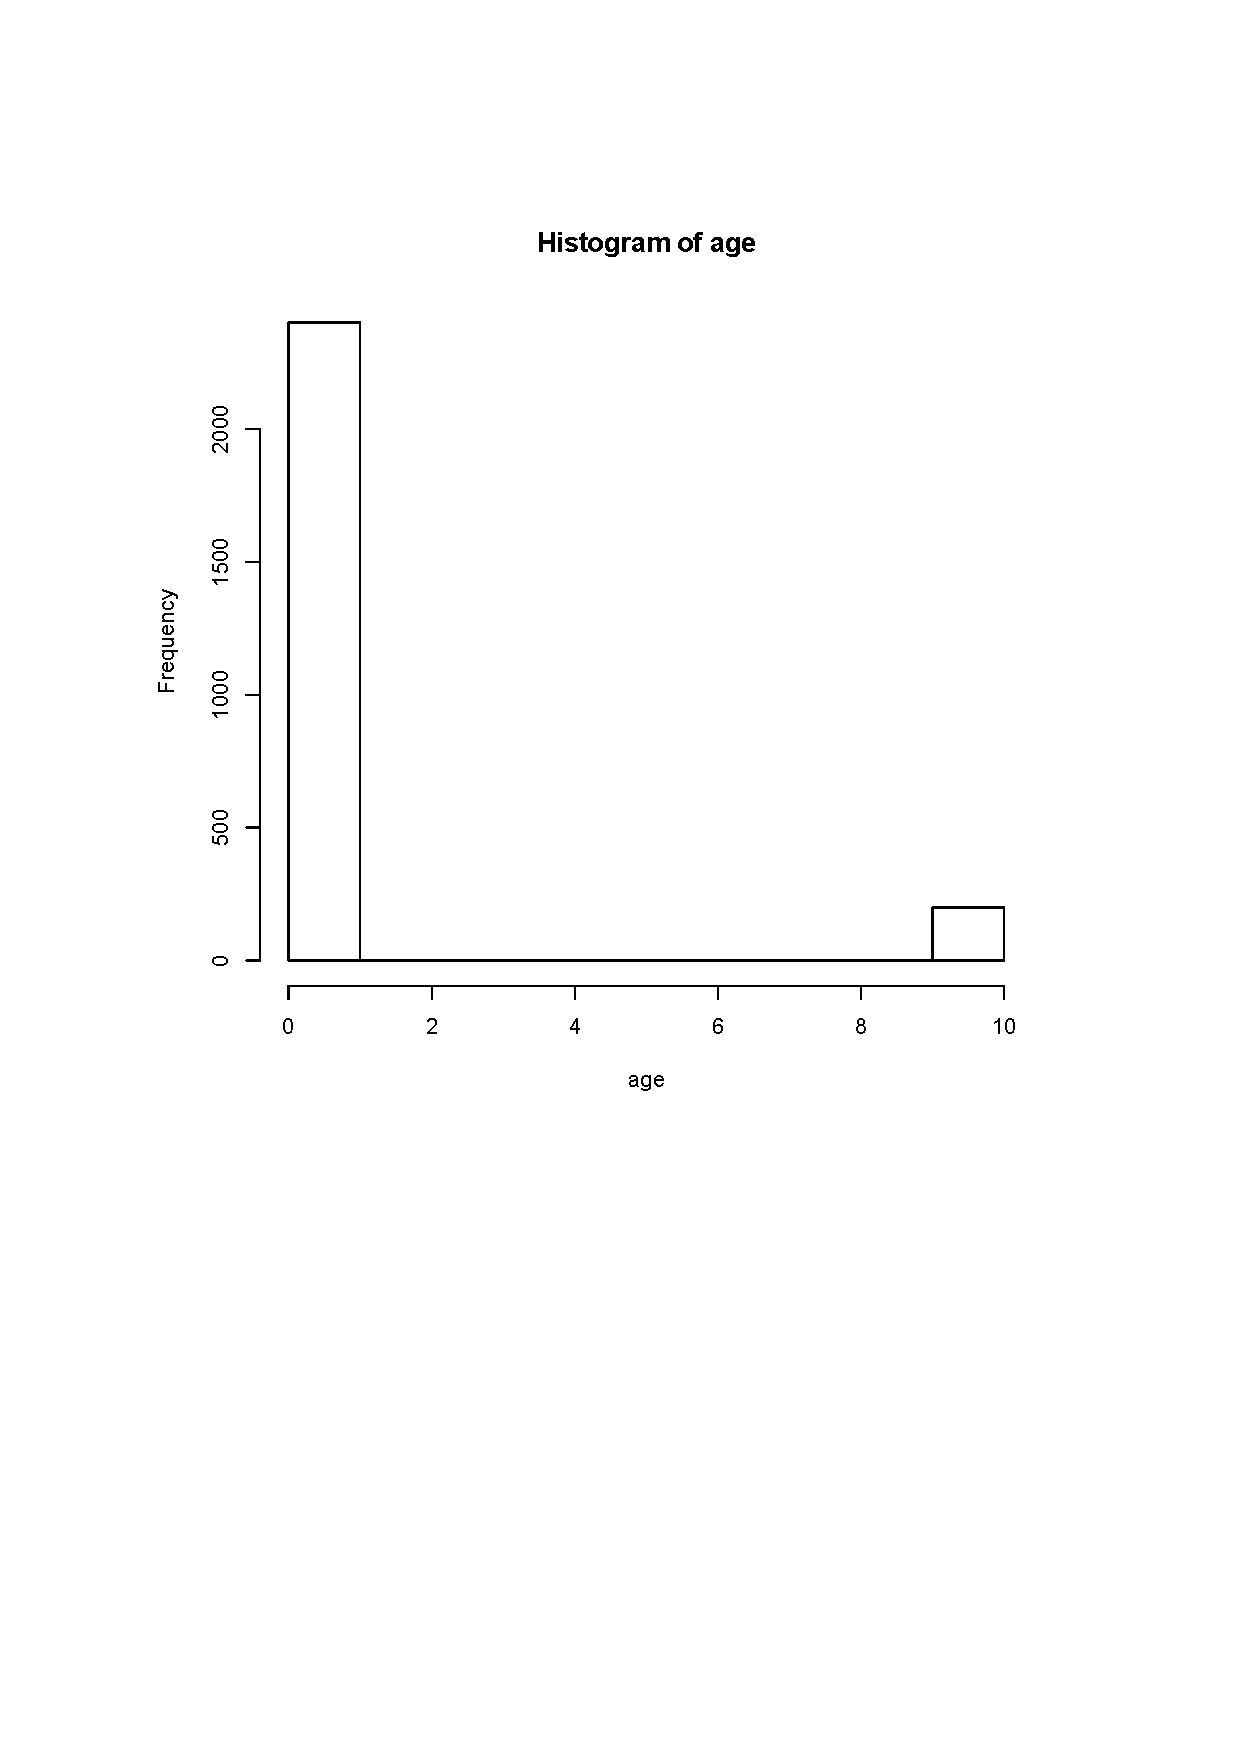
\epsfig{file=D0,width=5cm}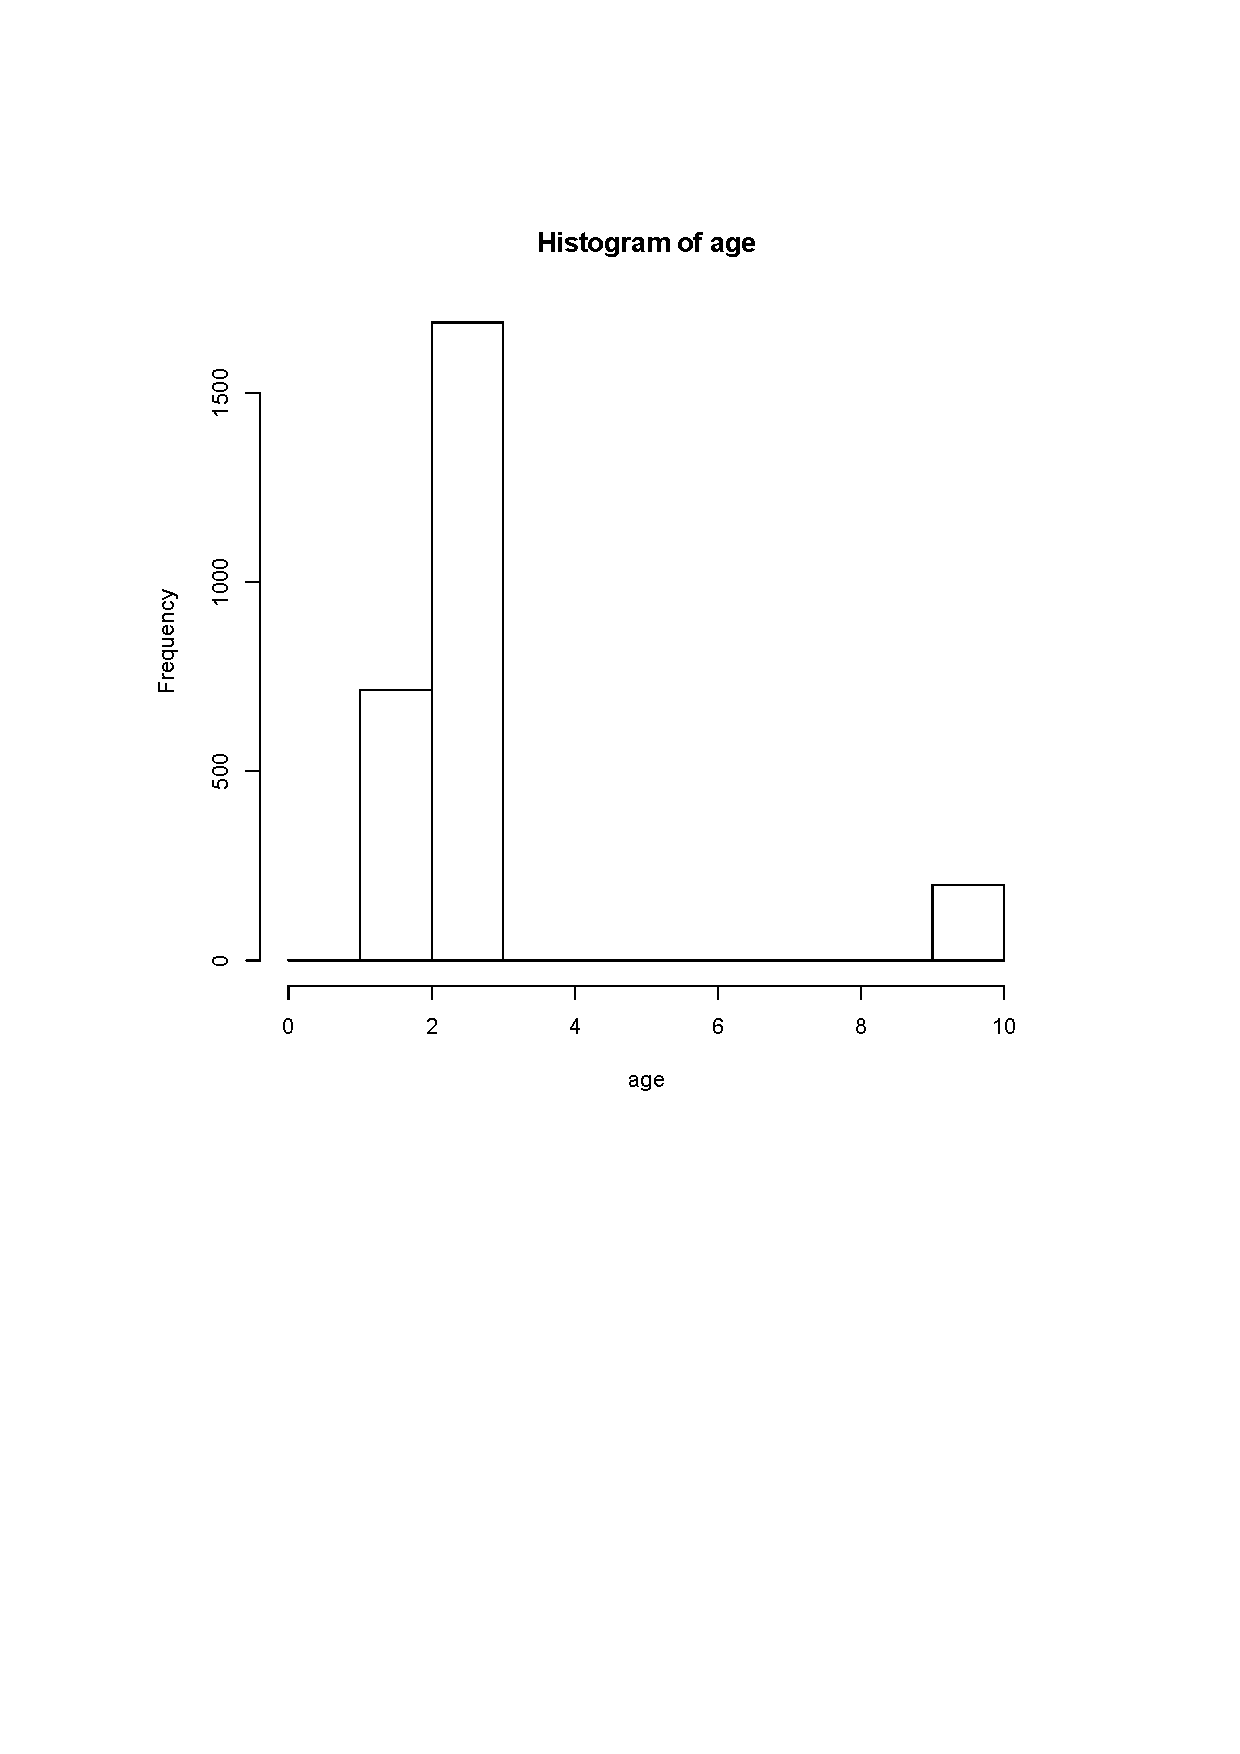
\epsfig{file=D1,width=5cm}\\
     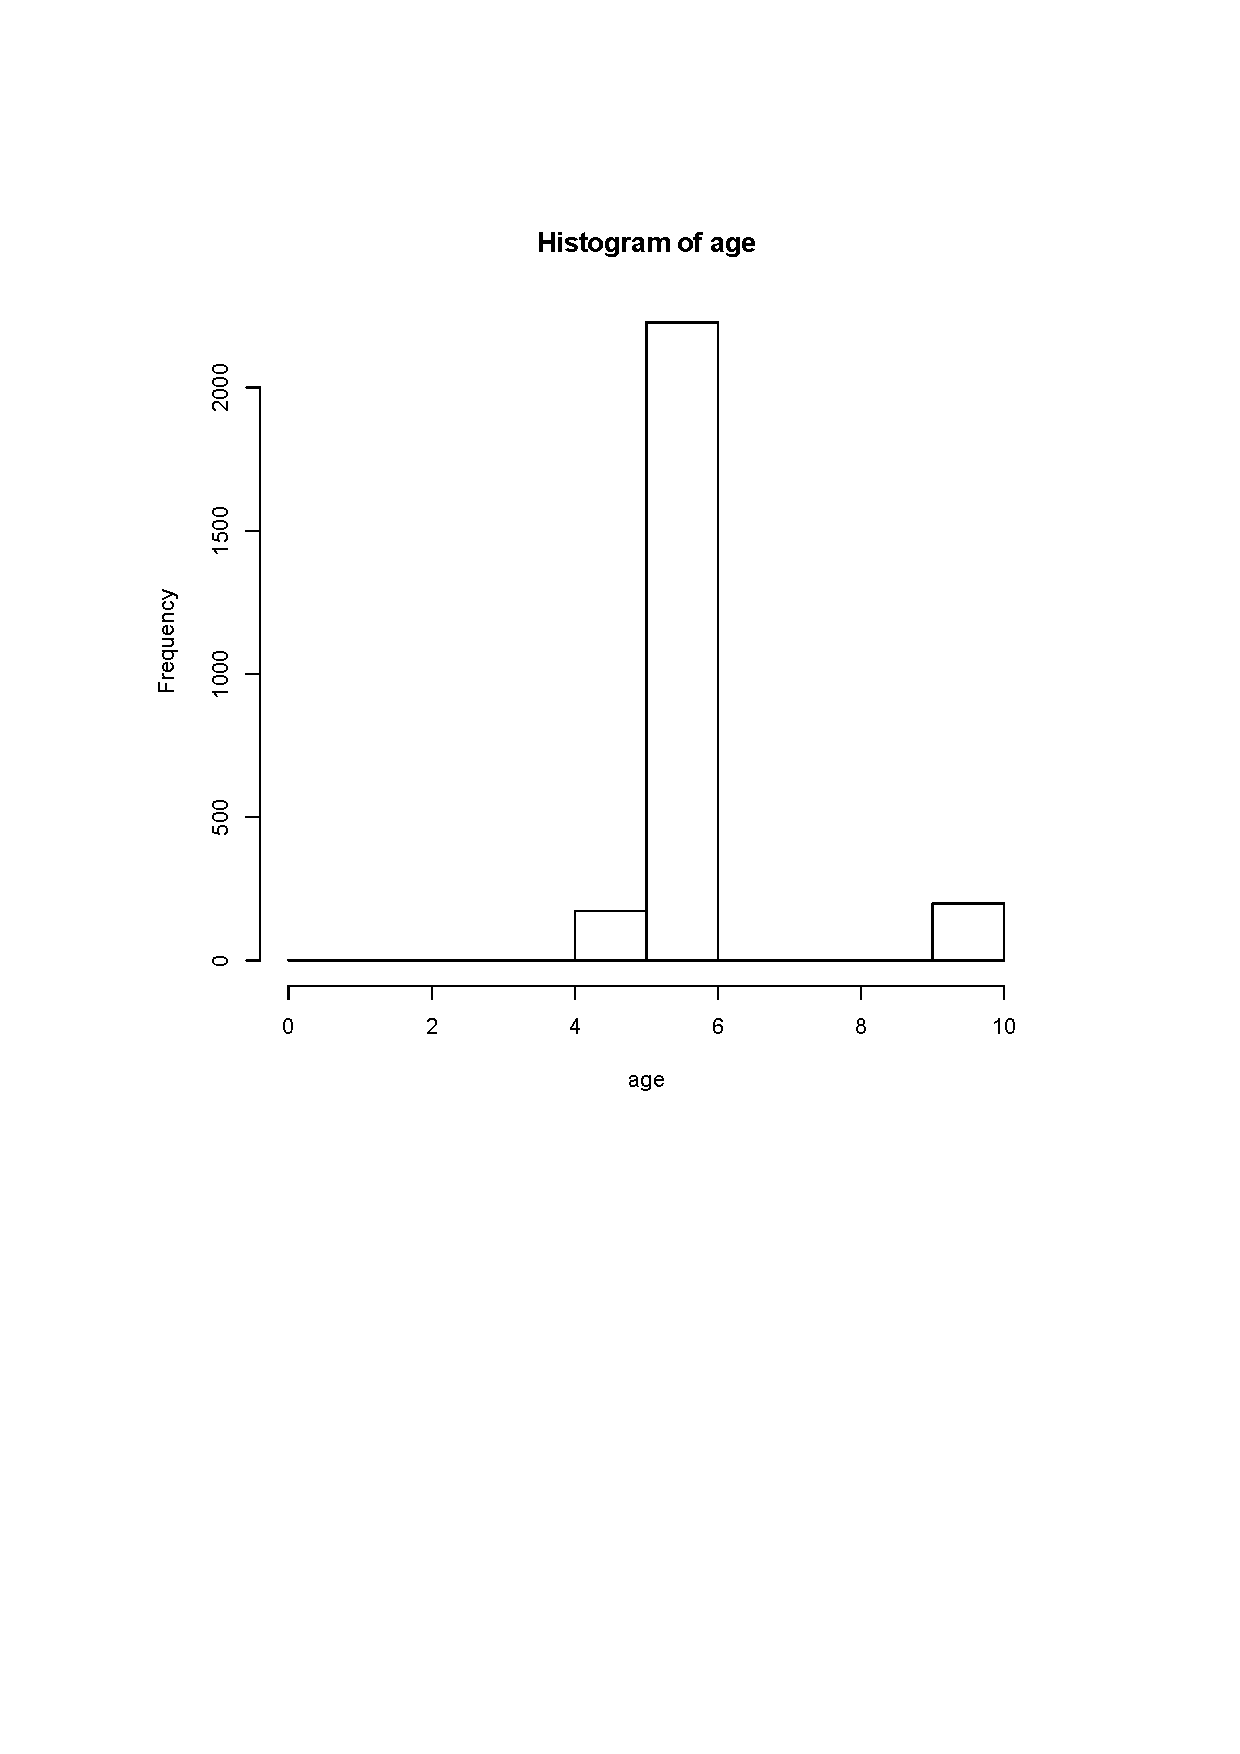
\epsfig{file=D2,width=5cm}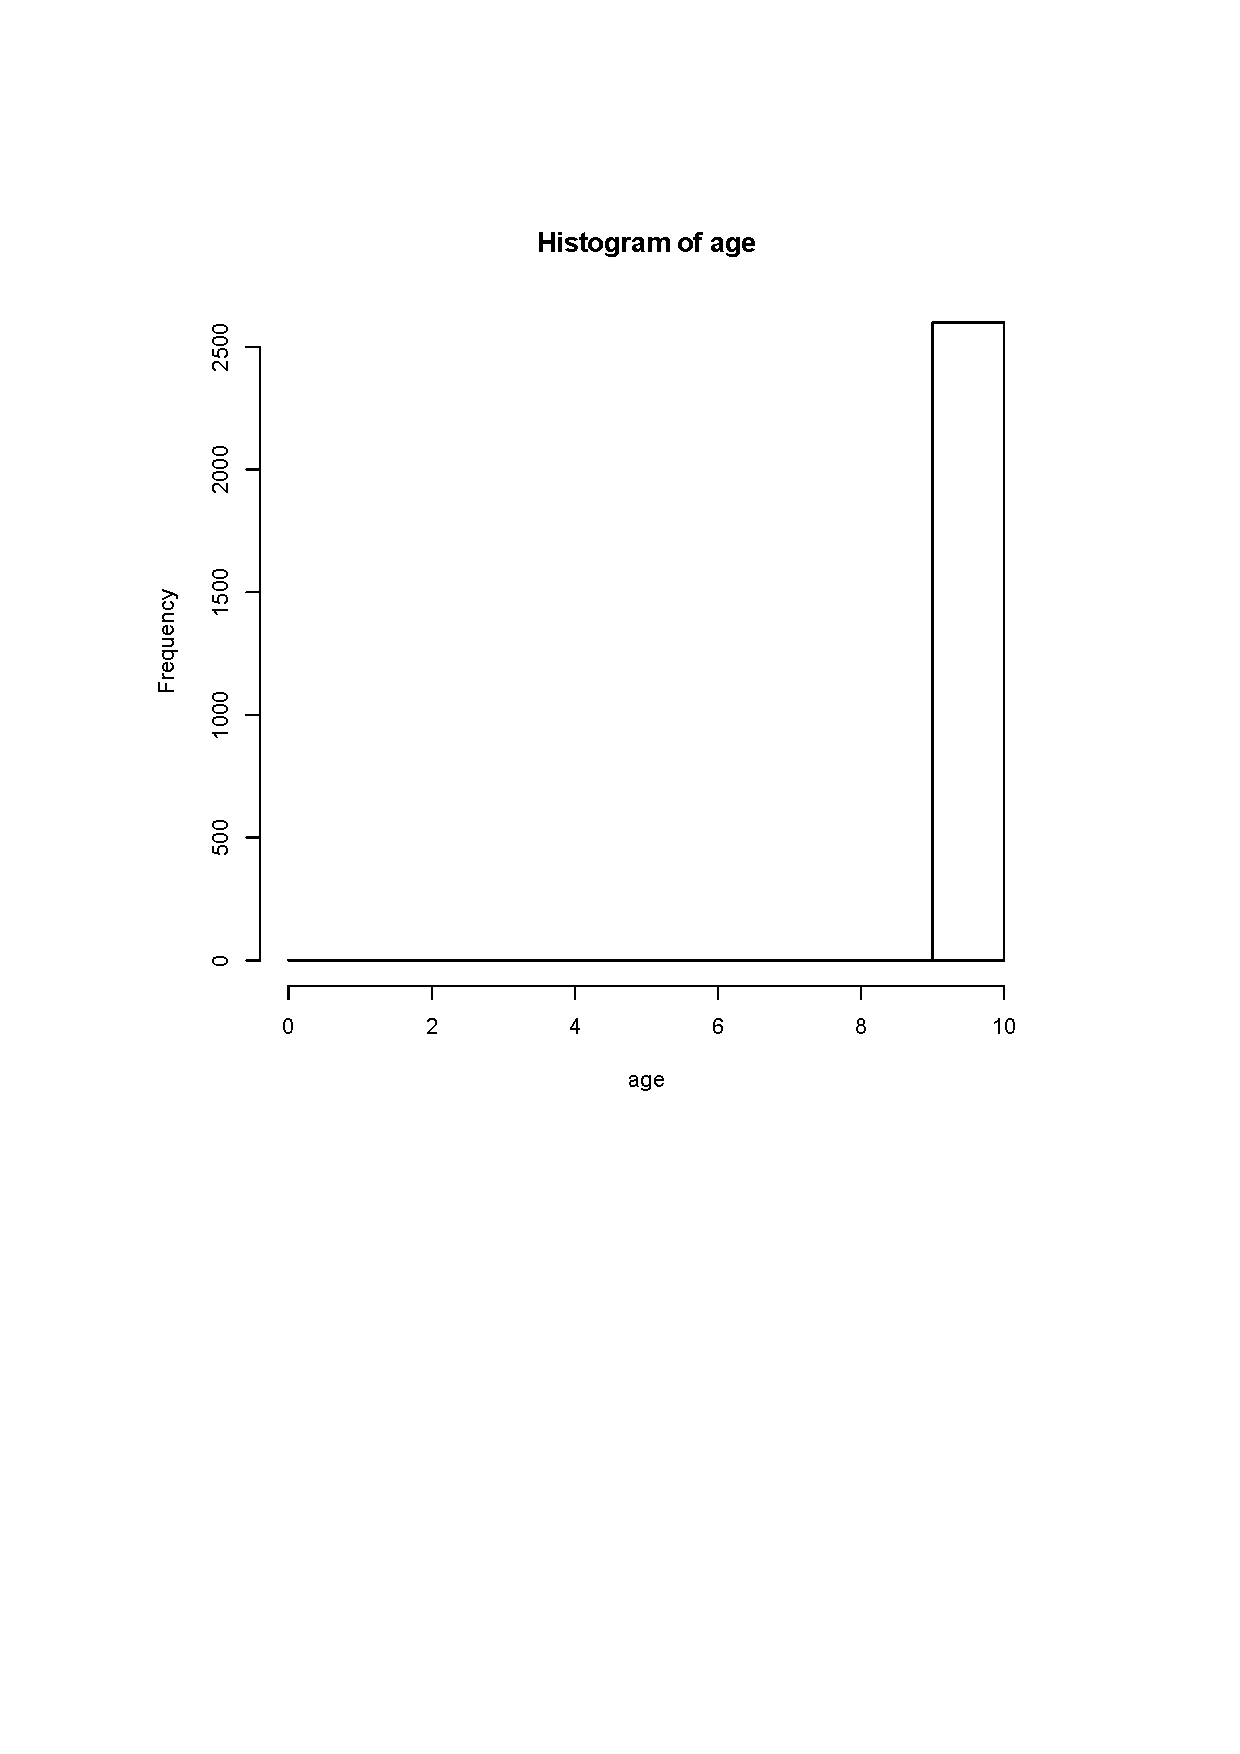
\epsfig{file=D3,width=5cm}\\
     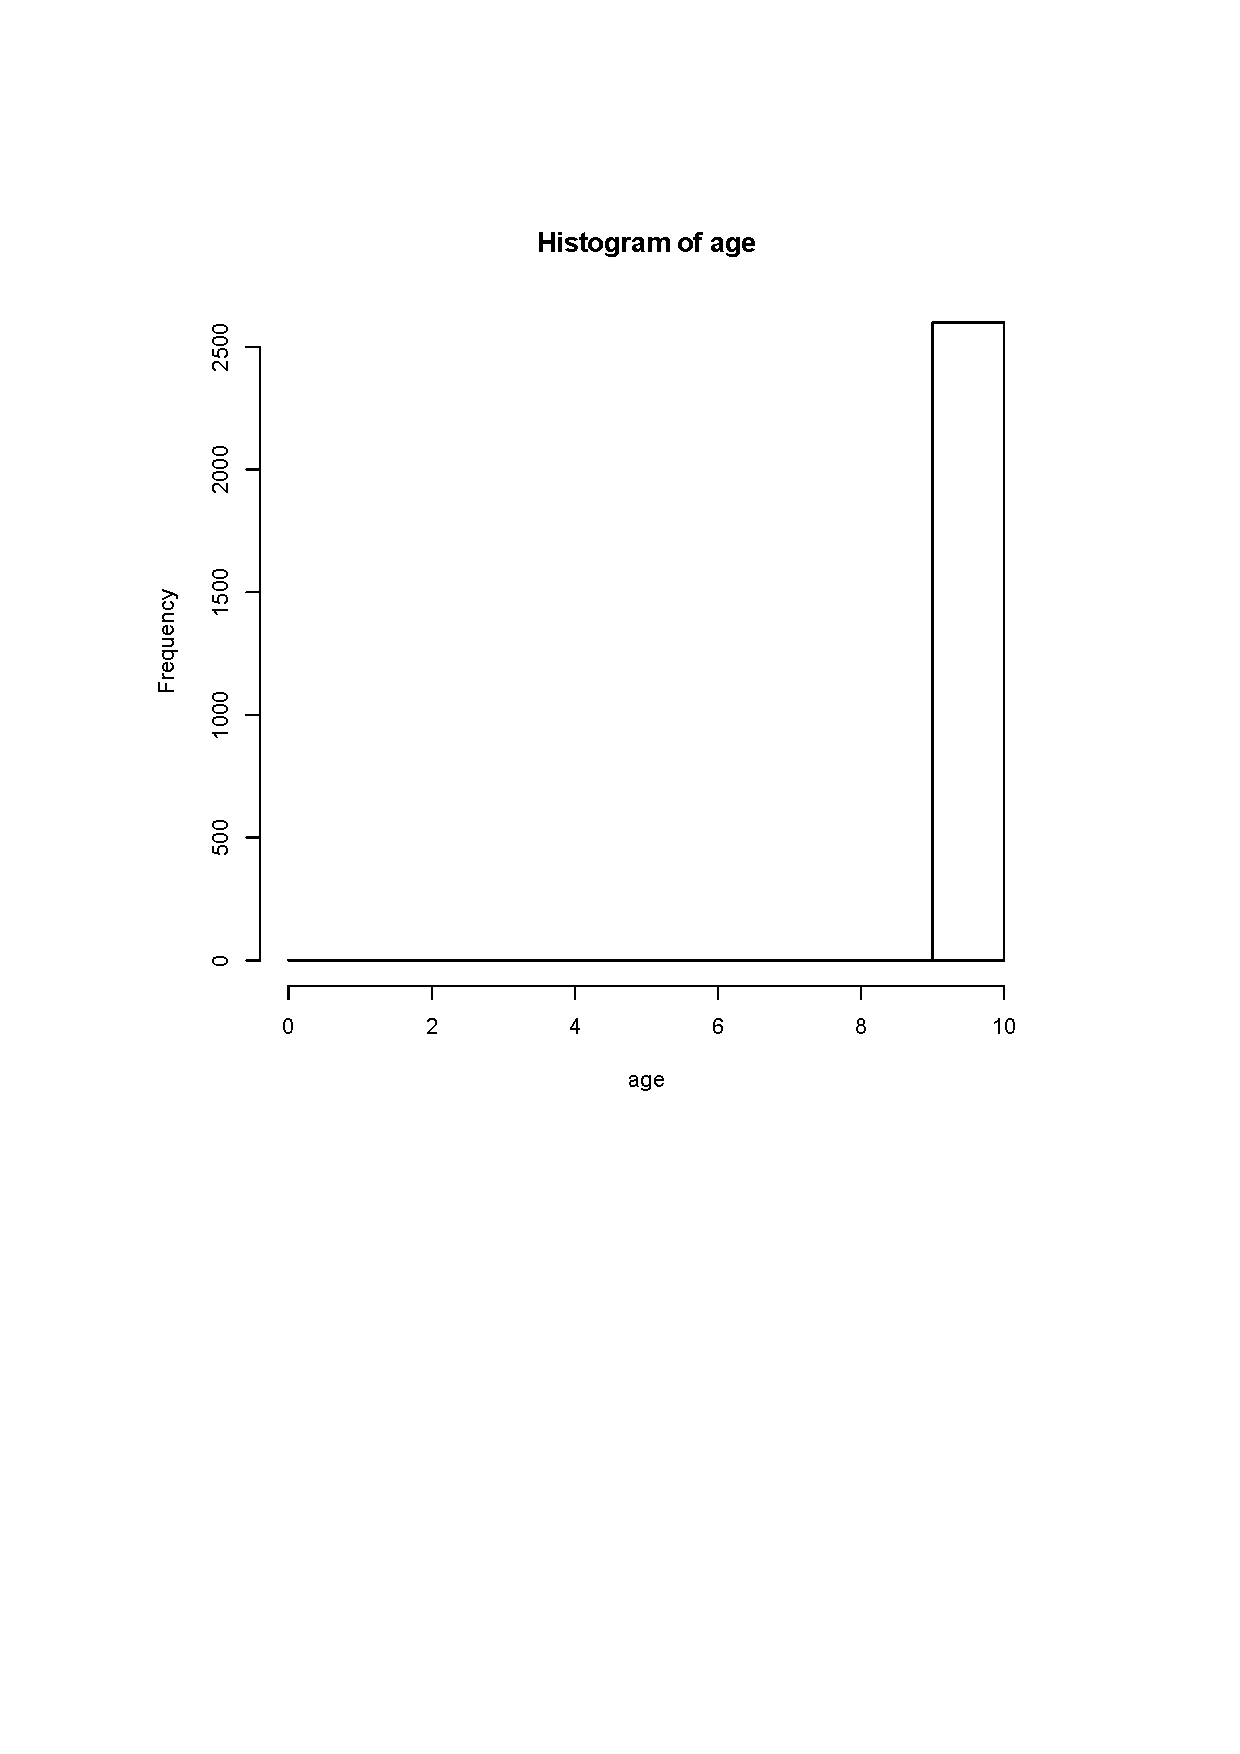
\epsfig{file=D4,width=5cm}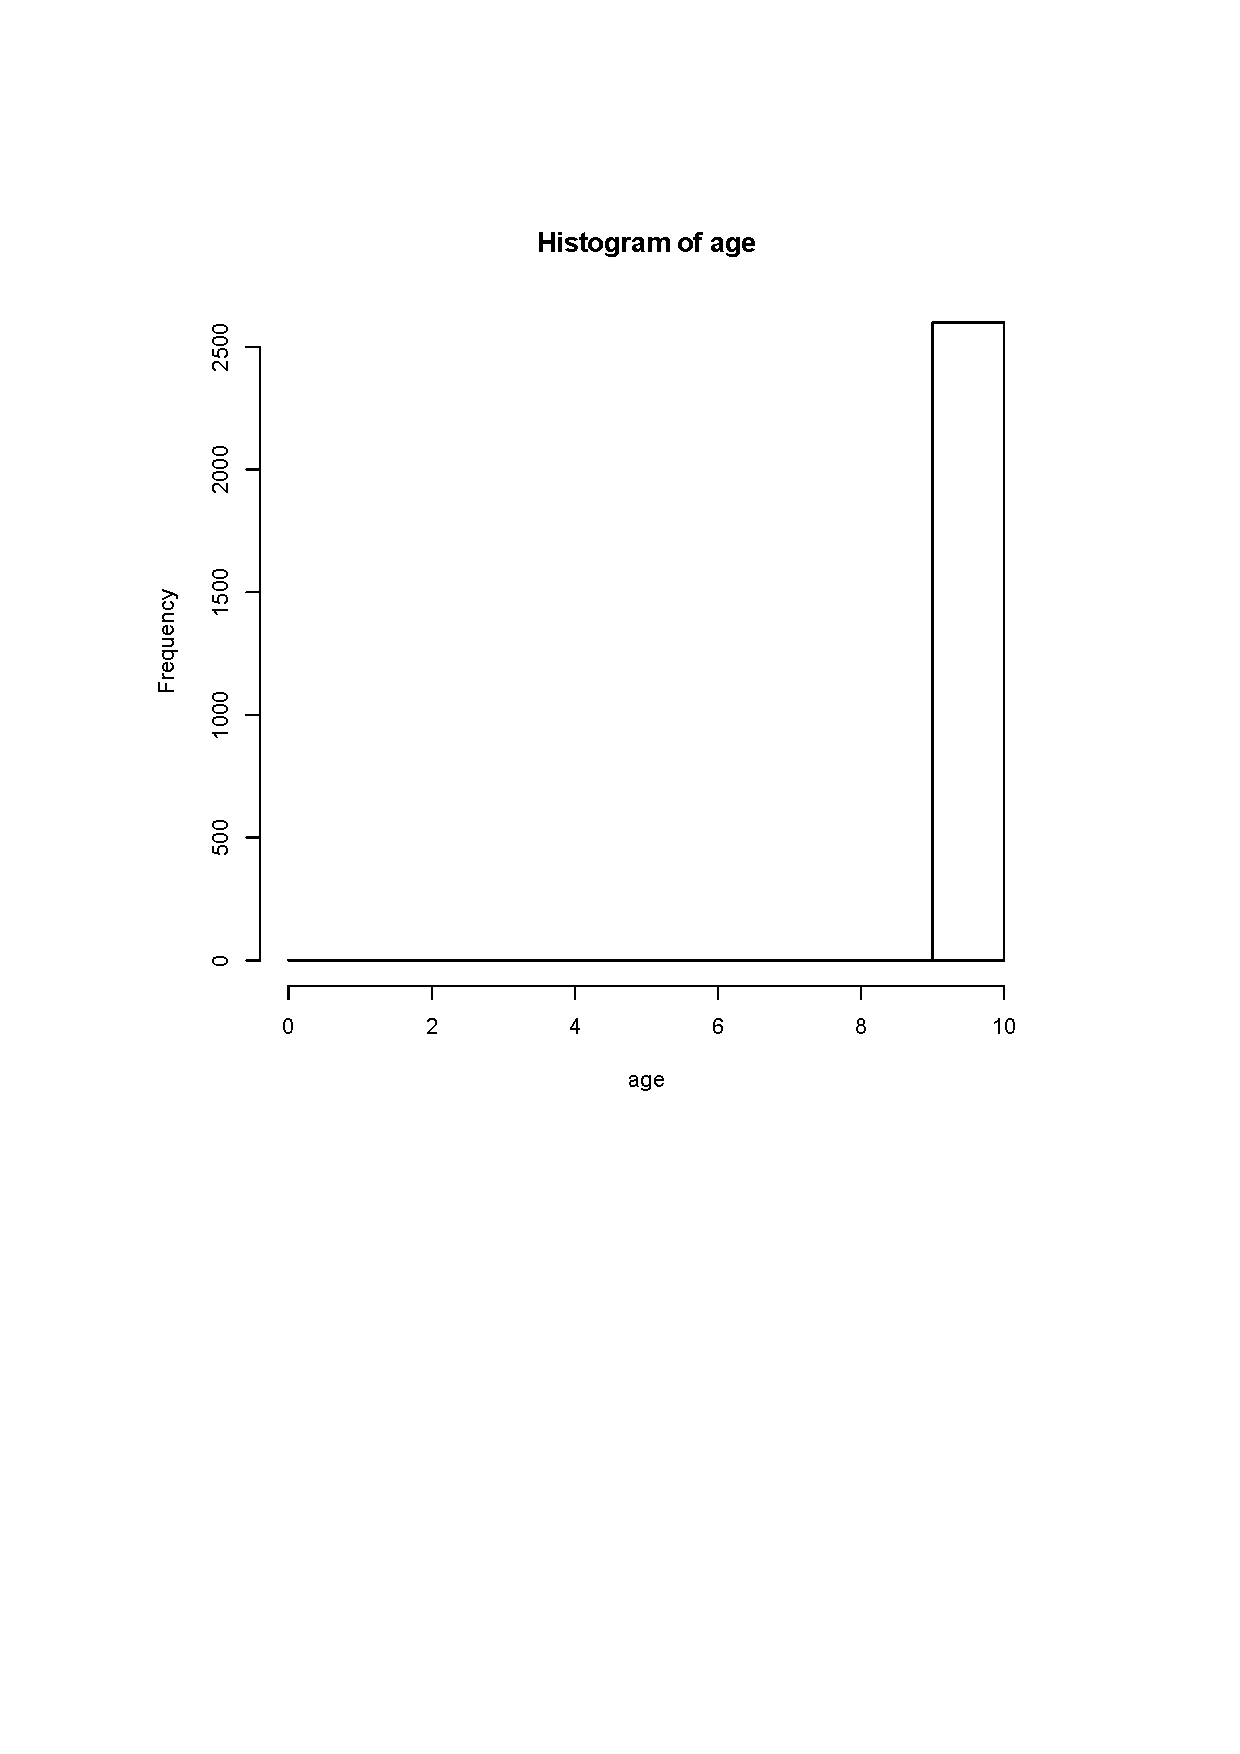
\epsfig{file=D5,width=5cm}\\
   \caption{Computed He apatite age distributitions obtained with PECUBE at t=0, 1, 2, 3, 4 and 5 Ma.}
   \label{fig:Detrital}
\end{figure}

\bibliographystyle{apalike}

\bibliography{../../Documents/Latex/abbreviatedjournalnames,../../Documents/Latex/references}

\end{document} 